\section{An initial overview of power electronics}
%\part{An initial overview of power electronics}
\title[Initial overview]{An initial overview of power electronics}  

\begin{frame}[plain]
    \titlepage
\end{frame}


%%%%%%%%%%%%%%%%%%%%%%%%%%%%%%%%%%%%%%%%%%%%%%%%%%%%%%%%%%%%%
%% What are power electronics? %%
%%%%%%%%%%%%%%%%%%%%%%%%%%%%%%%%%%%%%%%%%%%%%%%%%%%%%%%%%%%%%
\begin{frame}
	\frametitle{What are power electronics?}
		\vspace{0.5cm}
		\begin{figure}
		\begin{tikzpicture}[auto, node distance=1cm and 2cm]
			\draw
				node [input, name = input] {}
				node [block, right = of input] (pc) {Power converter}
				node [block, right = of pc] (load) {Load}
				node [block, below = of pc] (controller) {Controller}
				node [input, left = of controller, name = ref] {};
			\draw [->] (input) -- node  {$u_\mathrm{in}, i_\mathrm{in}$} (pc);
			\draw [->] (pc) -- node [name=M]  {$u_\mathrm{out}, i_\mathrm{out}$} (load);
			\draw [->] (ref) -- node  {Reference} (controller);
			\draw[->] (M) |- (controller);
			\draw[->] (controller) -- node {Feedback} (pc);
			\node[dot] at (M.south) {}; 
			% brace decoration right from entire plots
			\draw [decorate,decoration={brace,amplitude=10pt,mirror,raise=4pt},yshift=0pt] (8.75,-2.65) -- (8.75,0.5) node [black,midway, anchor = west, xshift = 0.5cm] {
				\begin{circuitikz}
					\node[twoportsplitshape, scale = 1.5](tp){};
					\draw (tp.left up) to [short, -o, i_<= $i_\mathrm{in}$] ++(-0.75,0) coordinate(tpin1)
					(tp.left down) to [short, -o] ++(-0.75,0) coordinate(tpin2);
					\draw[->] ([xshift=-0.9cm]tp.left up) to node[anchor = east]{$u_\mathrm{in}$} ([xshift=-0.9cm]tp.left down);
					\draw (tp.right up) to [short, -o, i= $i_\mathrm{out}$] ++(0.75,0) coordinate(tpout1)
					(tp.right down) to [short, -o] ++(+0.75,0) coordinate(tpout2);
					\draw[->] ([xshift=1cm]tp.right up) to node[anchor = west]{$u_\mathrm{out}$} ([xshift=1cm]tp.right down);
				\end{circuitikz}	
			};
		\end{tikzpicture}
		\caption{High-level block diagram of a power electronic system}
		\label{fig:power_electronics_block_diagram}
	\end{figure}
	\begin{varblock}[0.9\textwidth]{Power electronics -- a definition}
		Power electronics is a multidisciplinary branch of electrical engineering. It focuses on processing, controlling, and converting electric power. Power electronics manipulate voltages and currents to deliver a defined power to electrical equipment and devices.
	\end{varblock}
\end{frame}

%%%%%%%%%%%%%%%%%%%%%%%%%%%%%%%%%%%%%%%%%%%%%%%%%%%%%%%%%%%%%
%% Power electronics vs. microelectronics %%
%%%%%%%%%%%%%%%%%%%%%%%%%%%%%%%%%%%%%%%%%%%%%%%%%%%%%%%%%%%%%
\begin{frame}
	\frametitle{Power electronics vs. microelectronics}
		\vspace{0.5cm}
		\begin{figure}
		\begin{tikzpicture}[auto, node distance=1cm and 2cm]
			\matrix[column sep=0.03\textwidth, row sep=0.5cm]{
				\draw
					node [input, name = input, label=left:{Control signals}] {}
					node [block, right = of input, minimum width = 3.5cm] (pc) {Power electronics}
					node [output, right = of pc, name = output, label=right:{Output power}] {}
					node [input, above = of pc, name = control, label=above:{Control signals}] {};
				\draw [->] (input) --  (pc);
				\draw [->] (pc) -- (output);
				\draw [->] (control) -- (pc);
			\\
				\draw
					node [input, name = input, label=left:{Input signals}] {}
					node [block, right = of input, minimum width = 3.5cm] (pc) {Microelectronics}
					node [output, right = of pc, name = output, label=right:{Output signals}] {}
					node [input, below = of pc, name = control, label=below:{Power supply}] {};
				\draw [->] (input) --  (pc);
				\draw [->] (pc) -- (output);
				\draw [->] (control) -- (pc);
			\\
			};			
		\end{tikzpicture}
		\caption{Power electronics vs. microelectronics}
		\label{fig:power_electronics_vs_microelectronics}
	\end{figure}
\end{frame}


%%%%%%%%%%%%%%%%%%%%%%%%%%%%%%%%%%%%%%%%%%%%%%%%%%%%%%%%%%%%%
%% Power electronic tasks %%
%%%%%%%%%%%%%%%%%%%%%%%%%%%%%%%%%%%%%%%%%%%%%%%%%%%%%%%%%%%%%
\begin{frame}[c]
	\frametitle{Typical voltage and current manipulation tasks of power electronics}
	\begin{figure}
		\centering
		\begin{tikzpicture}[ampersand replacement=\&]
			\matrix[column sep=0.03\textwidth, row sep=0.5cm]{
			\begin{axis}[
				width=0.3\textwidth,
				height=0.4\textheight,
				axis lines=middle,
				xlabel={$\omega t$},
				ylabel={$u(\omega t)$},
				xlabel style={yshift=.0*\pgfkeysvalueof{/pgfplots/major tick length},
				anchor=west,
				inner xsep=0pt,
				xshift=0.5*\pgfkeysvalueof{/pgfplots/major tick length}},
				ylabel style={yshift=1.5*\pgfkeysvalueof{/pgfplots/major tick length},
				anchor=north west,
				inner ysep=0pt},
				xmin=0, xmax=2*pi,
				ymin=-1.5, ymax=1.5,
				xtick={0,1.57,3.14,4.71,6.28},
				xticklabels={$0$,$\frac{\pi}{2}$,$\pi$,$\frac{3\pi}{2}$,$2\pi$},
				ytick={-1,0,1},
				yticklabels={$-\hat{u}$,$0$,$\hat{u}$},
				grid=both,
				]
				\addplot[domain=0:2*pi, samples=100, signalblue, thick]{1};
			\end{axis}
			\&
			\begin{axis}[
				width=0.3\textwidth,
				height=0.4\textheight,
				axis lines=middle,
				xlabel={$\omega t$},
				ylabel={$u(\omega t)$},
				xlabel style={yshift=.0*\pgfkeysvalueof{/pgfplots/major tick length},
				anchor=west,
				inner xsep=0pt,
				xshift=0.5*\pgfkeysvalueof{/pgfplots/major tick length}},
				ylabel style={yshift=1.5*\pgfkeysvalueof{/pgfplots/major tick length},
				anchor=north west,
				inner ysep=0pt},
				xmin=0, xmax=2*pi,
				ymin=-1.5, ymax=1.5,
				xtick={0,1.57,3.14,4.71,6.28},
				xticklabels={$0$,$\frac{\pi}{2}$,$\pi$,$\frac{3\pi}{2}$,$2\pi$},
				ytick={-1,0,1},
				yticklabels={$-\hat{u}$,$0$,$\hat{u}$},
				grid=both,
				]
				\addplot[domain=0:2*pi, samples=100, signalblue, thick]{sin(deg(x))};
			\end{axis}
			\&
			\begin{axis}[
				width=0.3\textwidth,
				height=0.4\textheight,
				axis lines=middle,
				xlabel={$\omega t$},
				ylabel={$u(\omega t)$},
				xlabel style={yshift=.0*\pgfkeysvalueof{/pgfplots/major tick length},
				anchor=west,
				inner xsep=0pt,
				xshift=0.5*\pgfkeysvalueof{/pgfplots/major tick length}},
				ylabel style={yshift=1.5*\pgfkeysvalueof{/pgfplots/major tick length},
				anchor=north west,
				inner ysep=0pt},
				xmin=0, xmax=2*pi,
				ymin=-1.5, ymax=1.5,
				xtick={0,1.57,3.14,4.71,6.28},
				xticklabels={$0$,$\frac{\pi}{2}$,$\pi$,$\frac{3\pi}{2}$,$2\pi$},
				ytick={-1,0,1},
				yticklabels={$-\hat{u}$,$0$,$\hat{u}$},
				grid=both,
				]
				\addplot[domain=0:2*pi, samples=100, signalblue, thick]{sin(deg(x))};
			\end{axis}
			\\
			% add two arrows: one pointing up with a label "rectifier" and one pointing down with a label "inverter"
				\draw[->, thick] (1,0) -- (1,1);
				\node[anchor=east] at (1,0.5) {rectifier};
				\draw[->, thick] (2,1) -- (2,0);
				\node[anchor=west] at (2,0.5) {inverter};
			\&
				\draw[<->, thick] (1,0) -- (1,1);
				\node[anchor=east,  align=right] at (1,0.5) {frequency\\phase};
				\draw[<->, thick] (2,1) -- (2,0);
				\node[anchor=west] at (2,0.5) {amplitude};
			\&
				\draw[<->, thick] (1.5,0) -- (1.5,1);
				\node[anchor=east,  align=right] at (1.5,0.5) {number of\\phases};
			\\
			\begin{axis}[
				width=0.3\textwidth,
				height=0.4\textheight,
				axis lines=middle,
				xlabel={$\omega t$},
				ylabel={$u(\omega t)$},
				xlabel style={yshift=.0*\pgfkeysvalueof{/pgfplots/major tick length},
				anchor=west,
				inner xsep=0pt,
				xshift=0.5*\pgfkeysvalueof{/pgfplots/major tick length}},
				ylabel style={yshift=1.5*\pgfkeysvalueof{/pgfplots/major tick length},
				anchor=north west,
				inner ysep=0pt},
				xmin=0, xmax=2*pi,
				ymin=-1.5, ymax=1.5,
				xtick={0,1.57,3.14,4.71,6.28},
				xticklabels={$0$,$\frac{\pi}{2}$,$\pi$,$\frac{3\pi}{2}$,$2\pi$},
				ytick={-1,0,1},
				yticklabels={$-\hat{u}$,$0$,$\hat{u}$},
				grid=both,
				]
				\addplot[domain=0:2*pi, samples=100, signalblue, thick]{sin(deg(x))};
			\end{axis}
			\&
			\begin{axis}[
				width=0.3\textwidth,
				height=0.4\textheight,
				axis lines=middle,
				xlabel={$\omega t$},
				ylabel={$u(\omega t)$},
				xlabel style={yshift=.0*\pgfkeysvalueof{/pgfplots/major tick length},
				anchor=west,
				inner xsep=0pt,
				xshift=0.5*\pgfkeysvalueof{/pgfplots/major tick length}},
				ylabel style={yshift=1.5*\pgfkeysvalueof{/pgfplots/major tick length},
				anchor=north west,
				inner ysep=0pt},
				xmin=0, xmax=2*pi,
				ymin=-1.5, ymax=1.5,
				xtick={0,1.57,3.14,4.71,6.28},
				xticklabels={$0$,$\frac{\pi}{2}$,$\pi$,$\frac{3\pi}{2}$,$2\pi$},
				ytick={-1,0,1},
				yticklabels={$-\hat{u}$,$0$,$\hat{u}$},
				grid=both,
				]
				\addplot[domain=0:2*pi, samples=100, signalblue, thick]{0.5*sin(deg(2*x+pi/2))};
			\end{axis}
			\&
			\begin{axis}[
				width=0.3\textwidth,
				height=0.4\textheight,
				axis lines=middle,
				xlabel={$\omega t$},
				ylabel={$u(\omega t)$},
				xlabel style={yshift=.0*\pgfkeysvalueof{/pgfplots/major tick length},
				anchor=west,
				inner xsep=0pt,
				xshift=0.5*\pgfkeysvalueof{/pgfplots/major tick length}},
				ylabel style={yshift=1.5*\pgfkeysvalueof{/pgfplots/major tick length},
				anchor=north west,
				inner ysep=0pt},
				xmin=0, xmax=2*pi,
				ymin=-1.5, ymax=1.5,
				xtick={0,1.57,3.14,4.71,6.28},
				xticklabels={$0$,$\frac{\pi}{2}$,$\pi$,$\frac{3\pi}{2}$,$2\pi$},
				ytick={-1,0,1},
				yticklabels={$-\hat{u}$,$0$,$\hat{u}$},
				grid=both,
				]
				\addplot[domain=0:2*pi, samples=100, signalblue, thick]{sin(deg(x))};
				\addplot[domain=0:2*pi, samples=100, signalred, thick]{sin(deg(x-2*pi/3))};
				\addplot[domain=0:2*pi, samples=100, signalgreen, thick]{sin(deg(x+2*pi/3))};
			\end{axis}
			\\
			};
		\end{tikzpicture}
	\end{figure}
\end{frame}

%%%%%%%%%%%%%%%%%%%%%%%%%%%%%%%%%%%%%%%%%%%%%%%%%%%%%%%%%%%%%
%% Power electronic application examples: residential %%
%%%%%%%%%%%%%%%%%%%%%%%%%%%%%%%%%%%%%%%%%%%%%%%%%%%%%%%%%%%%%
\begin{frame}[c]
	\frametitle{Power electronic application examples: residential}
	\begin{figure}
		\centering
		\begin{subfigure}[b]{0.49\textwidth}
			\centering
			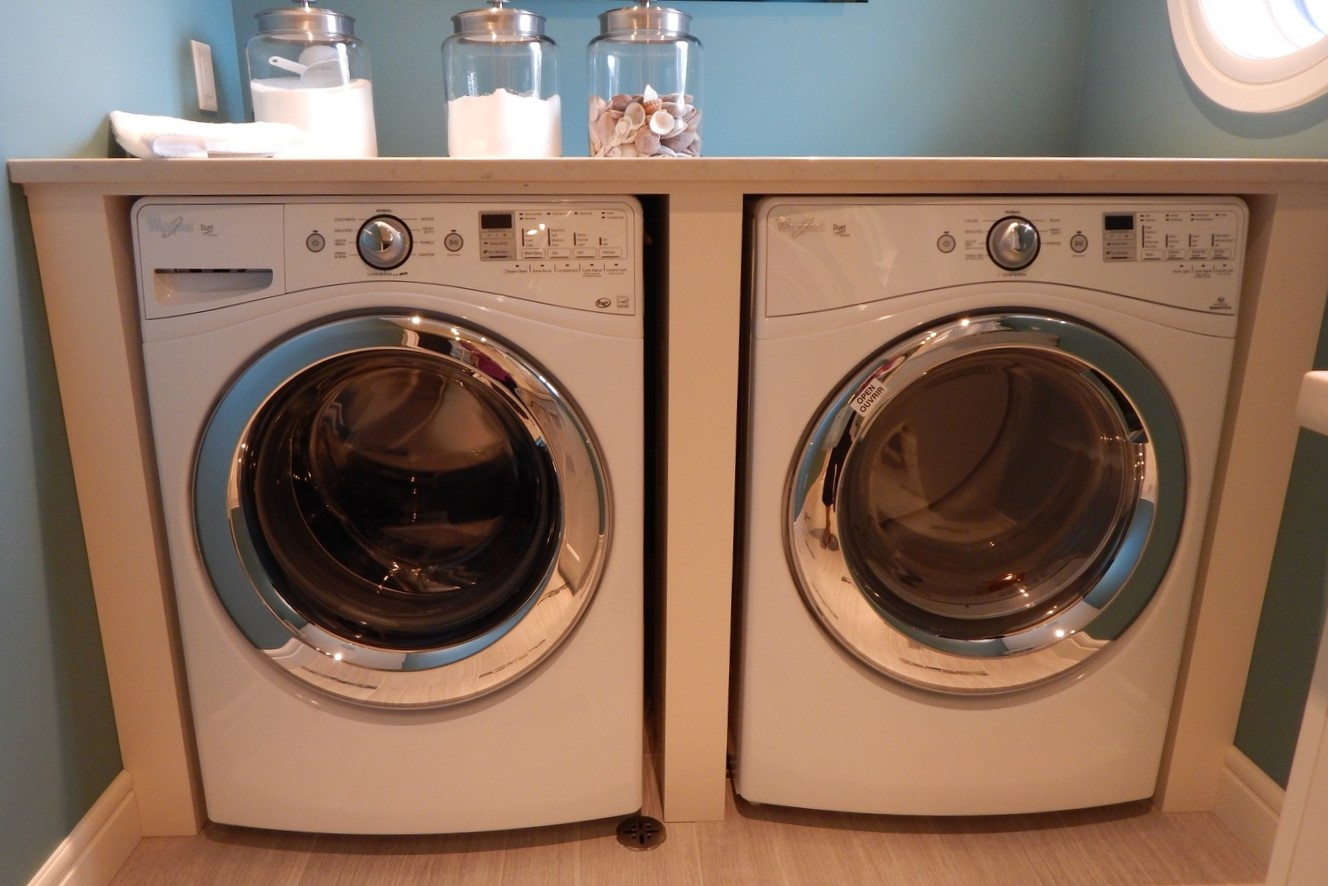
\includegraphics[width=0.5\textwidth]{fig/lec01/Home_appliance.jpg}
			\caption{Home appliances (source: \href{https://pxhere.com/de/photo/863012}{pxhere}, \href{https://creativecommons.org/publicdomain/zero/1.0/}{CC0~1.0})}
		\end{subfigure}
		\hfill
		\begin{subfigure}[b]{0.49\textwidth}
			\centering
			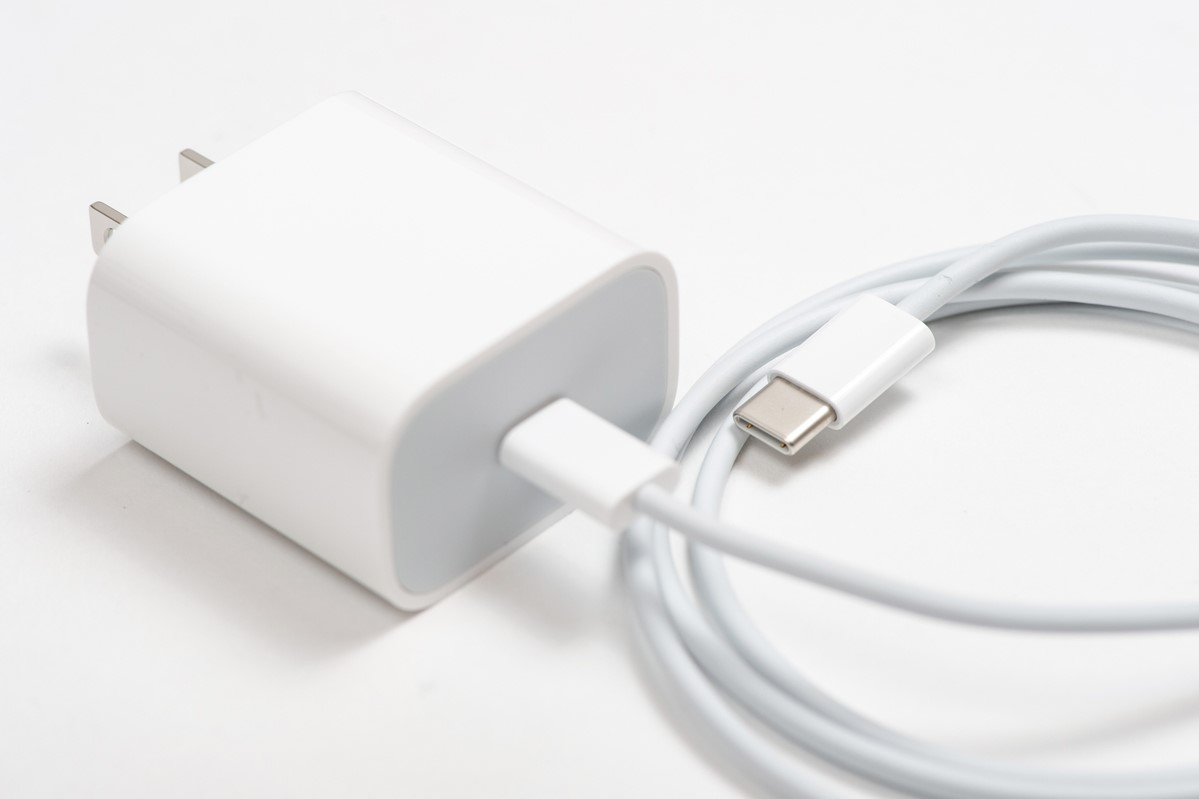
\includegraphics[width=0.5\textwidth]{fig/lec01/Smartphone_charger.jpg}
			\caption{Smartphone charger (source: \href{https://www.rawpixel.com/image/5923136/photo-image-phone-public-domain-white}{rawpixel}, \href{https://creativecommons.org/publicdomain/zero/1.0/}{CC0~1.0})}
		\end{subfigure}
		\\
		\begin{subfigure}[b]{0.49\textwidth}
			\centering
			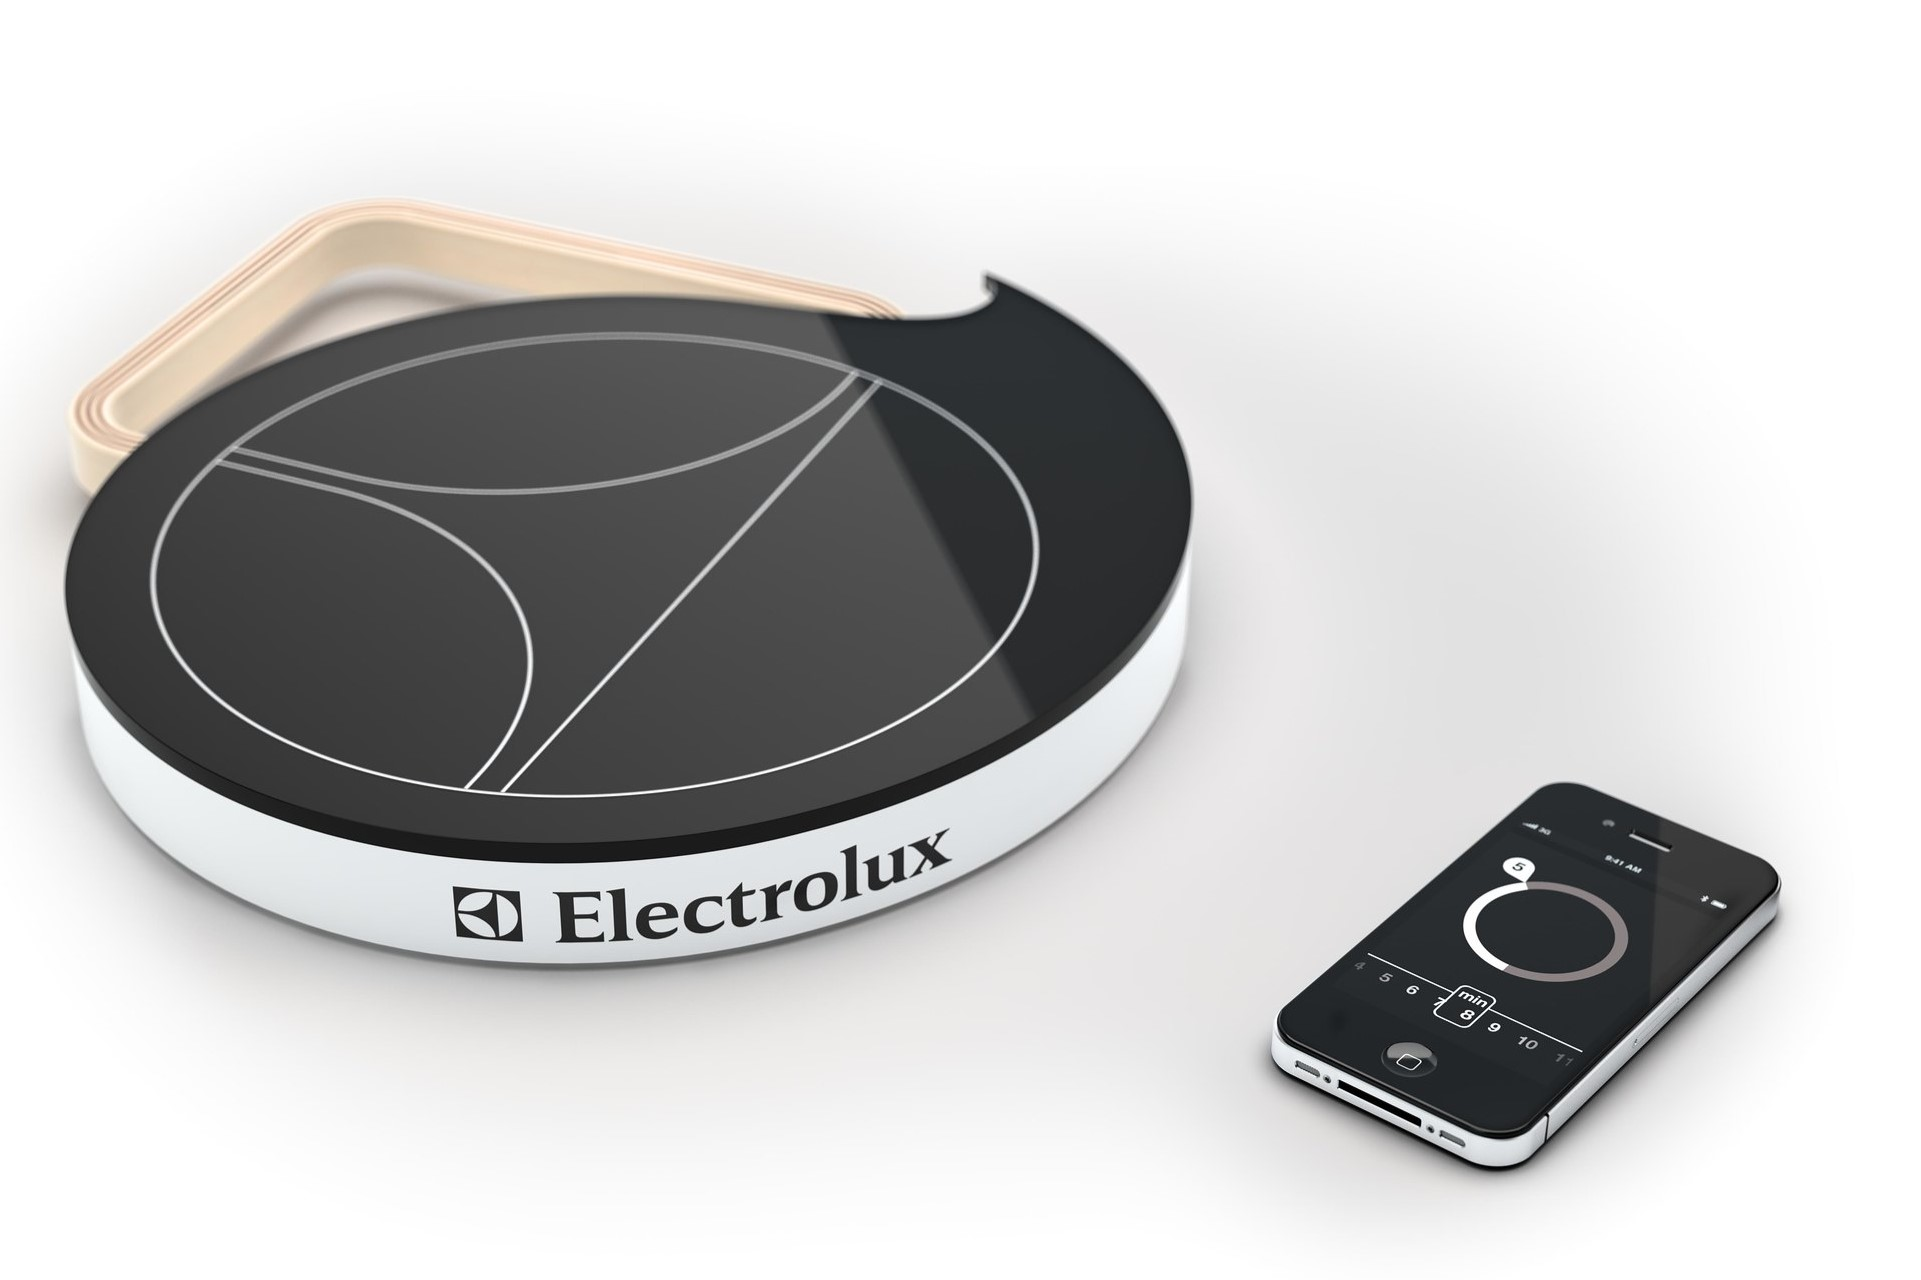
\includegraphics[width=0.5\textwidth]{fig/lec01/Induction_plate.jpg}
			\caption{Induction plate (source: \href{https://www.flickr.com/photos/electrolux-design-lab/6035618944}{flickr}, Electrolux, \href{https://creativecommons.org/licenses/by-nc/2.0/}{CC~BY-SA-NC~2.0})}
		\end{subfigure}
		\hfill
		\begin{subfigure}[b]{0.49\textwidth}
			\centering
			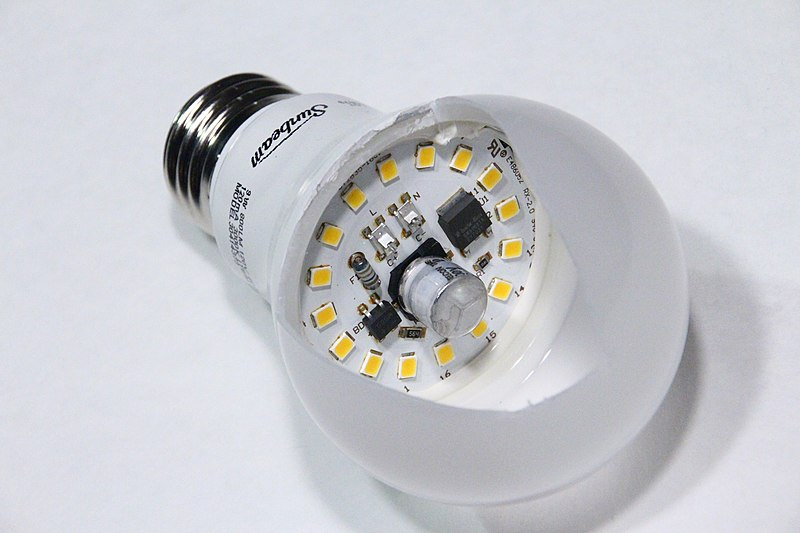
\includegraphics[width=0.5\textwidth]{fig/lec01/LED_light_bulb.jpg}
			\caption{LED rectifier (source: \href{https://commons.wikimedia.org/wiki/File:LED-E27-Light-Bulb-1134.jpg}{Wikimedia Commons}, D.~Tribble, \href{https://creativecommons.org/licenses/by-sa/4.0/deed.en}{CC~BY-SA~4.0})}
		\end{subfigure}
	\end{figure}
\end{frame}

%%%%%%%%%%%%%%%%%%%%%%%%%%%%%%%%%%%%%%%%%%%%%%%%%%%%%%%%%%%%%
%% Power electronic application examples: industrial %%
%%%%%%%%%%%%%%%%%%%%%%%%%%%%%%%%%%%%%%%%%%%%%%%%%%%%%%%%%%%%%
\begin{frame}[c]
	\frametitle{Power electronic application examples: industrial}
	\begin{figure}
		\centering
		\begin{subfigure}[b]{0.49\textwidth}
			\centering
			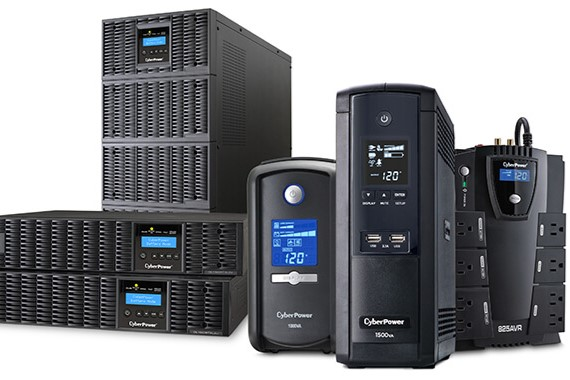
\includegraphics[width=0.5\textwidth]{fig/lec01/UPS.jpg}
			\caption{Uninterruptible power supply (source: \href{https://commons.wikimedia.org/wiki/File:CyberPower_UPS_Systems.jpg}{Wikimedia Commons}, Stevebwallace, \href{https://creativecommons.org/licenses/by-sa/4.0/deed.en}{CC~BY-SA~4.0})}
		\end{subfigure}
		\hfill
		\begin{subfigure}[b]{0.49\textwidth}
			\centering
			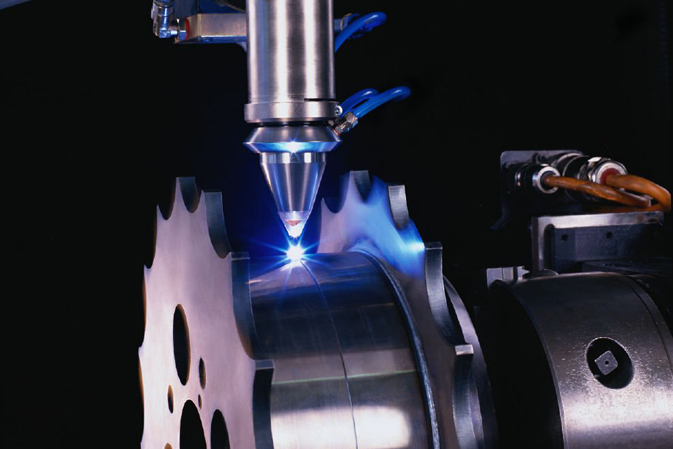
\includegraphics[width=0.5\textwidth]{fig/lec01/Welding.jpg}
			\caption{Welding power supply (source: \href{https://commons.wikimedia.org/wiki/File:Trumpf_laserschweissen.jpg}{Wikimedia Commons}, Trumpf GmbH, \href{https://creativecommons.org/licenses/by-sa/3.0/deed.en}{CC~BY-SA~3.0})}
		\end{subfigure}
		\\
		\begin{subfigure}[b]{0.49\textwidth}
			\centering
			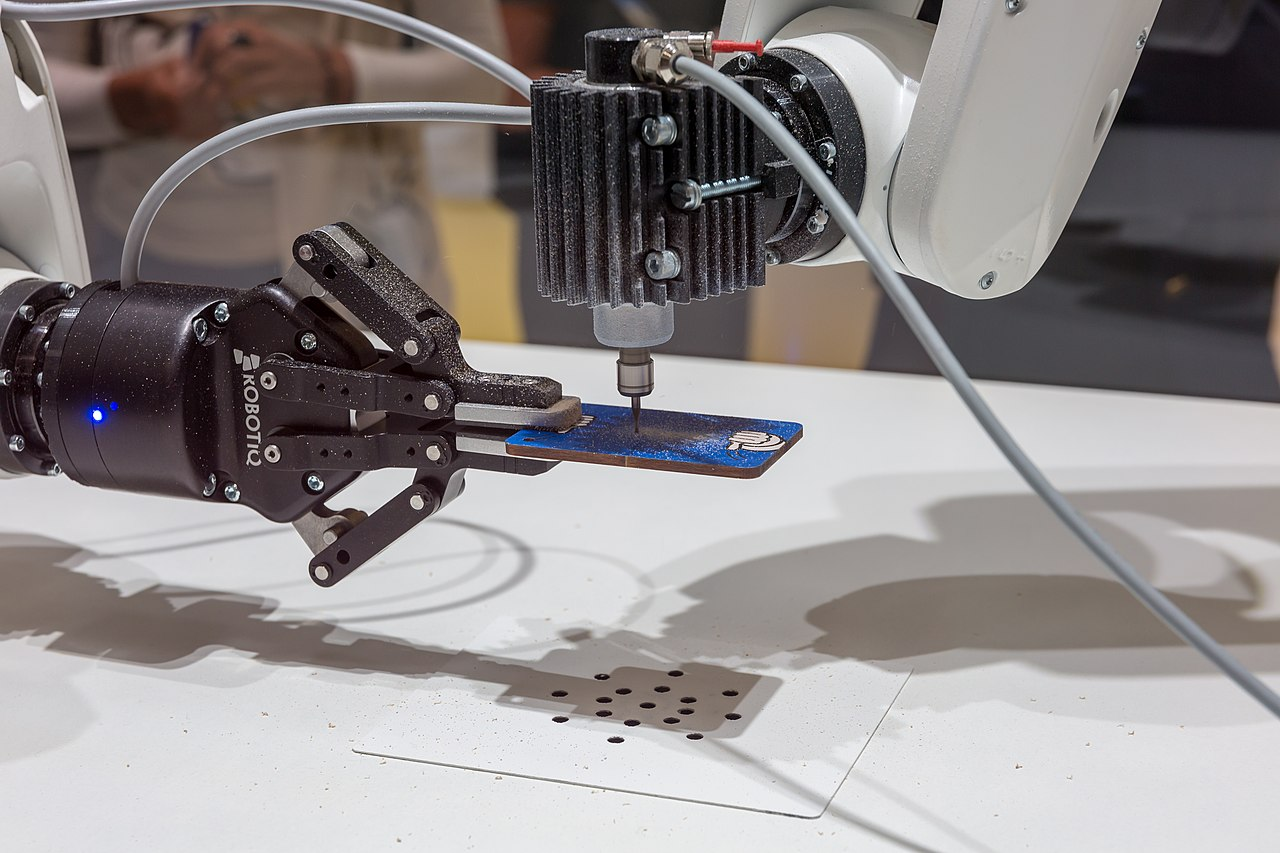
\includegraphics[width=0.5\textwidth]{fig/lec01/Robot.jpg}
			\caption{Industrial drives / automation (source: \href{https://de.m.wikipedia.org/wiki/Datei:Paris_Motor_Show_2018,_Paris_\%281Y7A1752\%29.jpg}{Wikimedia Commons}, M.~BLume, \href{https://creativecommons.org/licenses/by-sa/4.0/deed.de}{CC~BY-SA~4.0})}
		\end{subfigure}
		\hfill
		\begin{subfigure}[b]{0.49\textwidth}
			\centering
			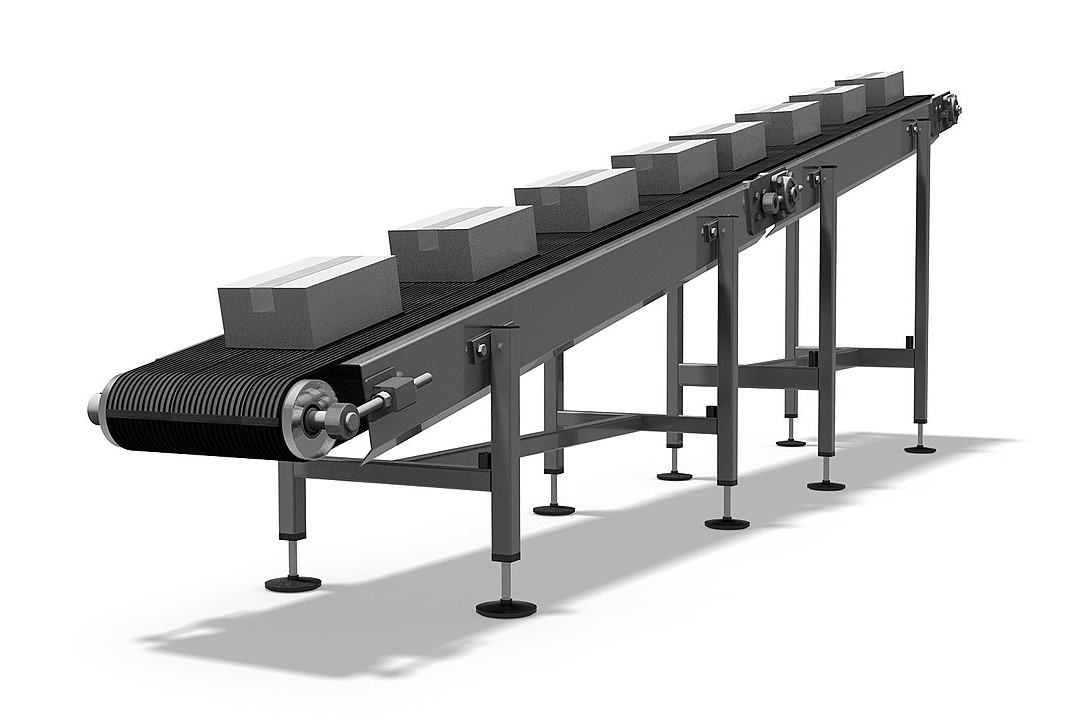
\includegraphics[width=0.5\textwidth]{fig/lec01/Conveyor.jpg}
			\caption{Conveyor belt drive (source: \href{https://commons.wikimedia.org/wiki/File:Inclined-belt_conveyor.jpgg}{Wikimedia Commons},  	K.~Hannessen, \href{https://creativecommons.org/licenses/by-sa/4.0/deed.en}{CC~BY-SA~4.0})}
		\end{subfigure}
	\end{figure}
\end{frame}

%%%%%%%%%%%%%%%%%%%%%%%%%%%%%%%%%%%%%%%%%%%%%%%%%%%%%%%%%%%%%
%% Power electronic application examples: energy system %%
%%%%%%%%%%%%%%%%%%%%%%%%%%%%%%%%%%%%%%%%%%%%%%%%%%%%%%%%%%%%%
\begin{frame}[c]
	\frametitle{Power electronic application examples: energy system}
	\begin{figure}
		\centering
		\begin{subfigure}[b]{0.49\textwidth}
			\centering
			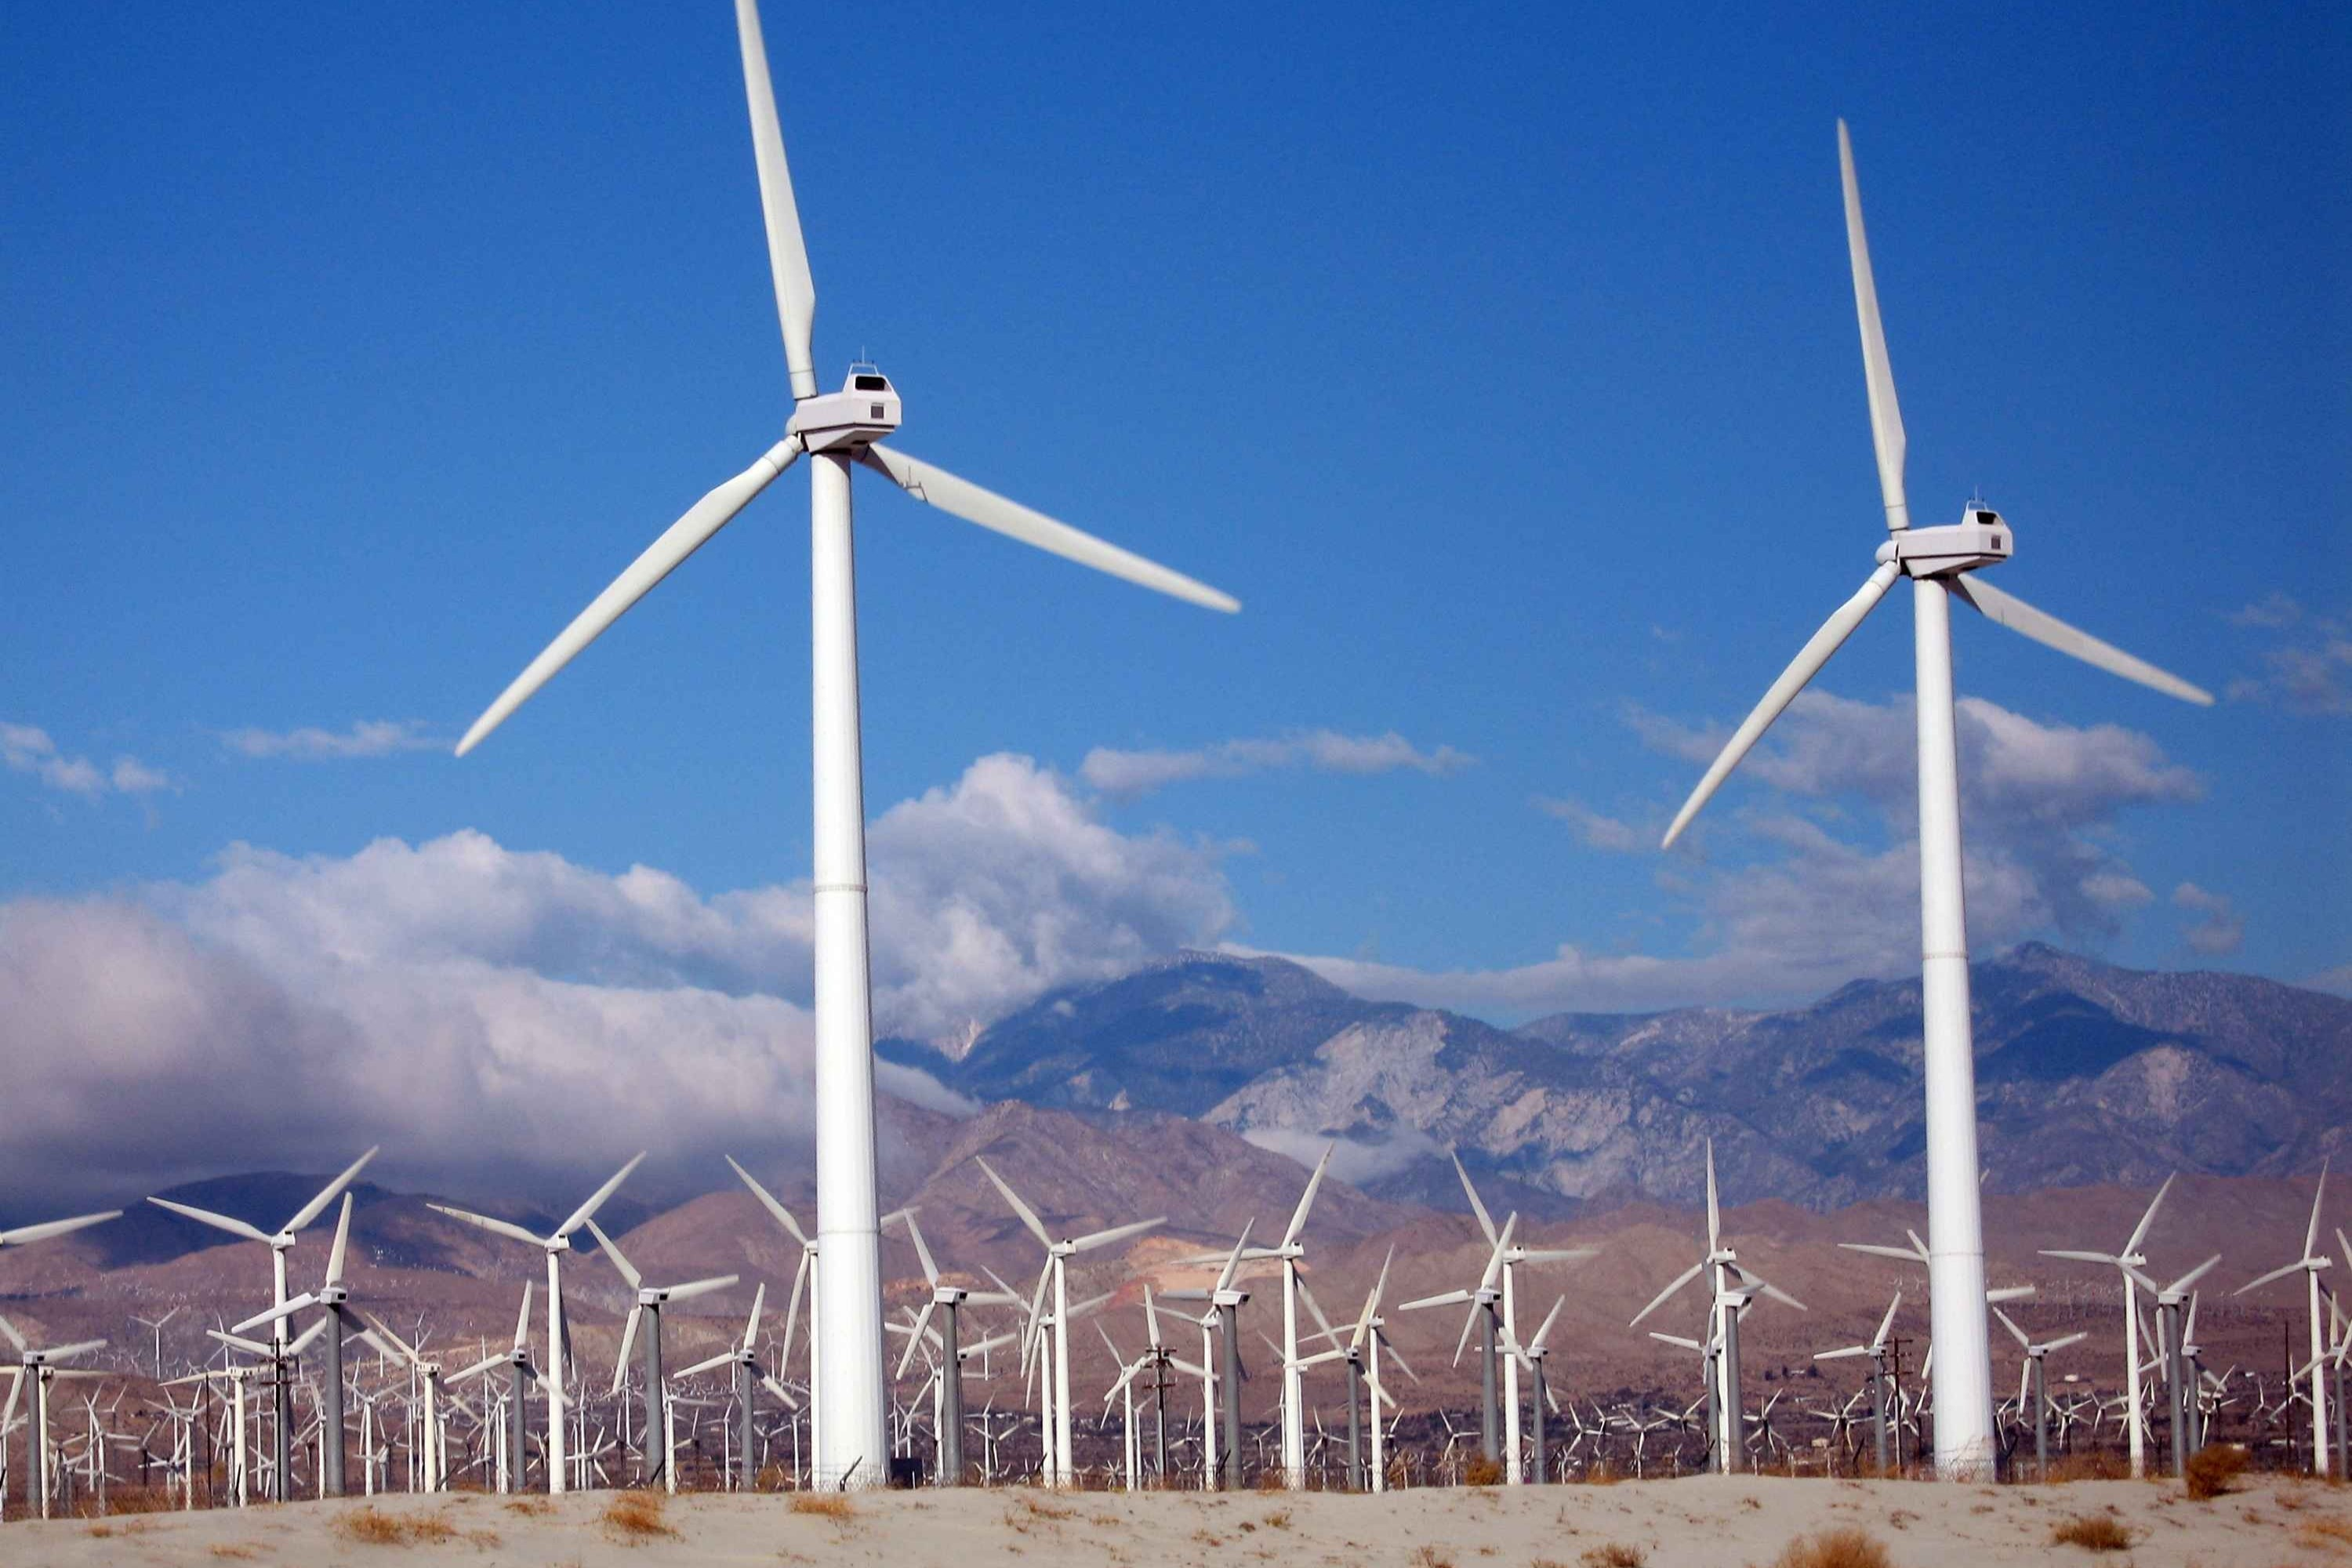
\includegraphics[width=0.5\textwidth]{fig/lec01/sky-farm-windmill.jpg}
			\caption{Wind power plants (source: \href{https://pxhere.com/en/photo/954757}{pxhere}, \href{https://creativecommons.org/publicdomain/zero/1.0/}{CC0~1.0})}
		\end{subfigure}
		\hfill
		\begin{subfigure}[b]{0.49\textwidth}
			\centering
			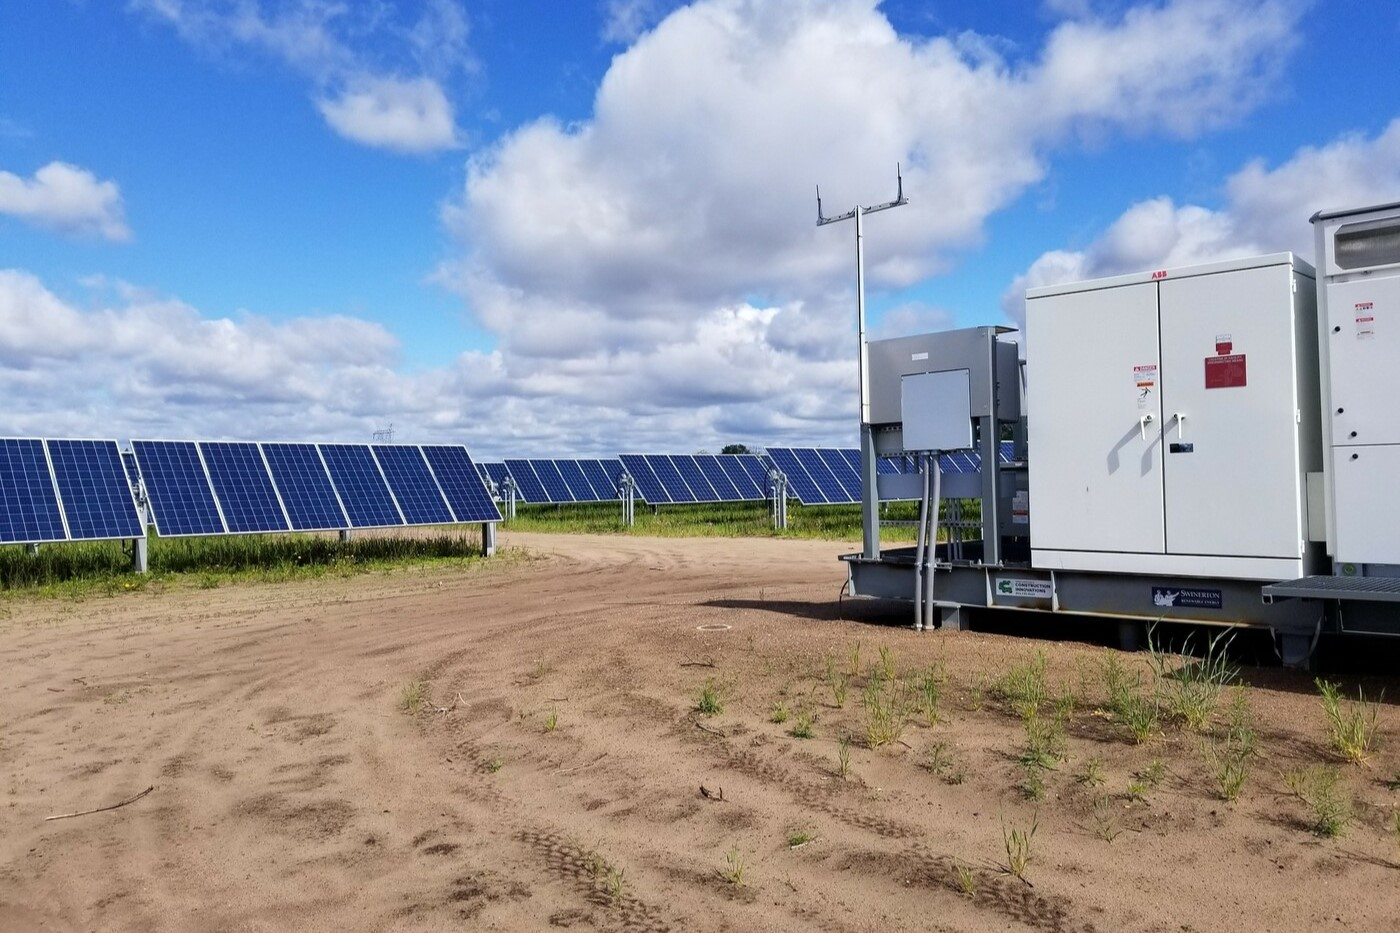
\includegraphics[width=0.5\textwidth]{fig/lec01/PV_field.jpg}
			\caption{PV power plants (source: \href{https://pxhere.com/en/photo/1685464}{pxhere}, \href{https://creativecommons.org/publicdomain/zero/1.0/}{CC0~1.0})}
		\end{subfigure}
		\\
		\begin{subfigure}[b]{0.49\textwidth}
			\centering
			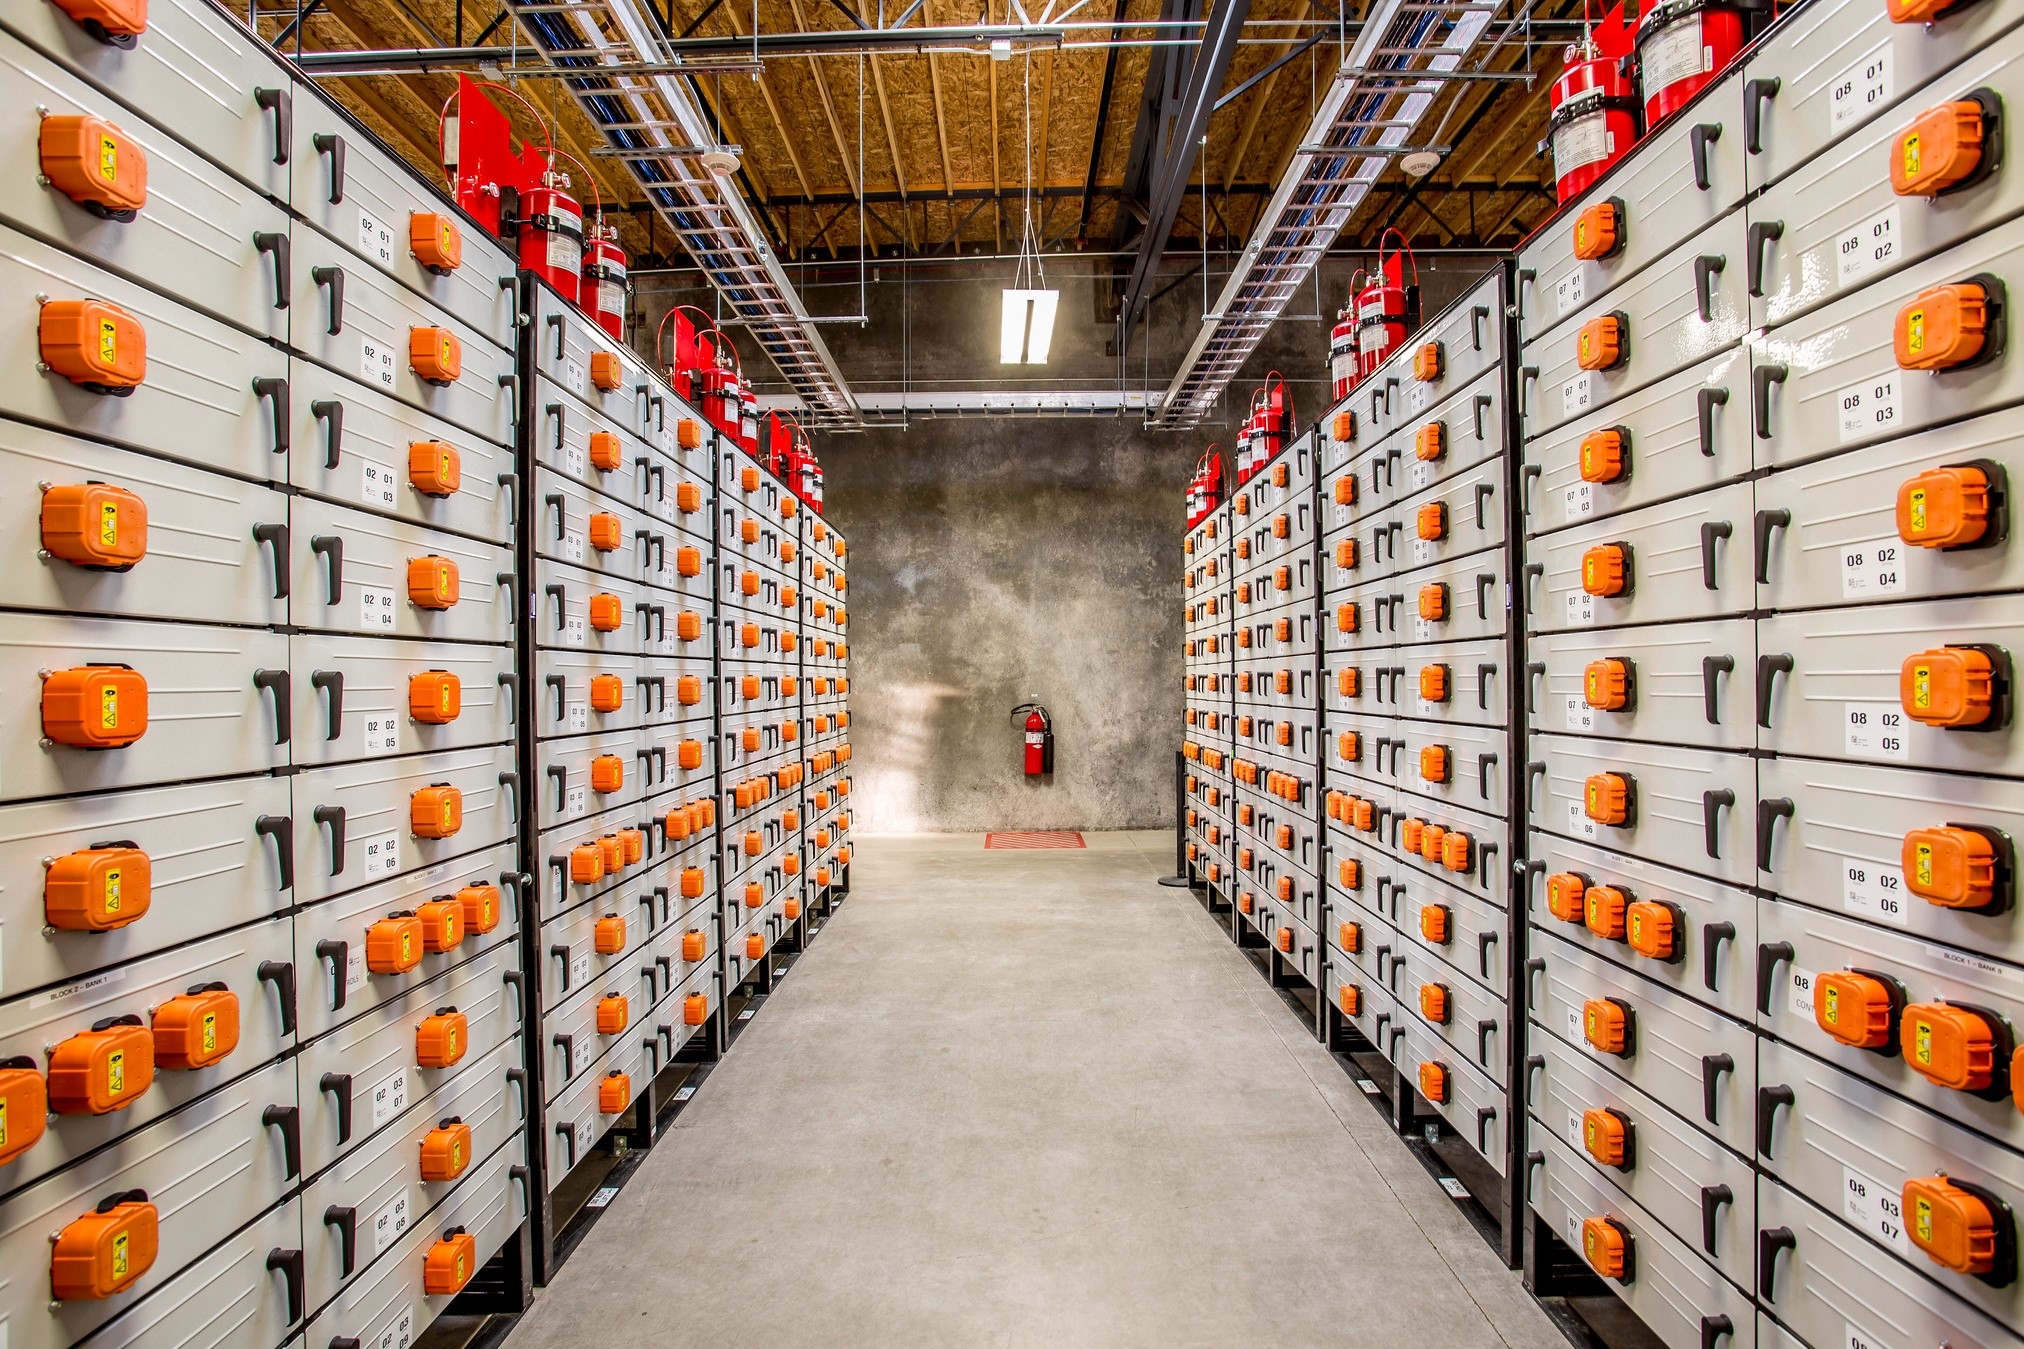
\includegraphics[width=0.5\textwidth]{fig/lec01/Battery_storage.jpg}
			\caption{Battery storage systems (source: \href{https://www.flickr.com/photos/portlandgeneralelectric/8905201835}{flickr}, 
			Portland General Electric, \href{https://creativecommons.org/licenses/by-nd/2.0/}{CC~BY-ND~2.0})}
		\end{subfigure}
		\hfill
		\begin{subfigure}[b]{0.49\textwidth}
			\centering
			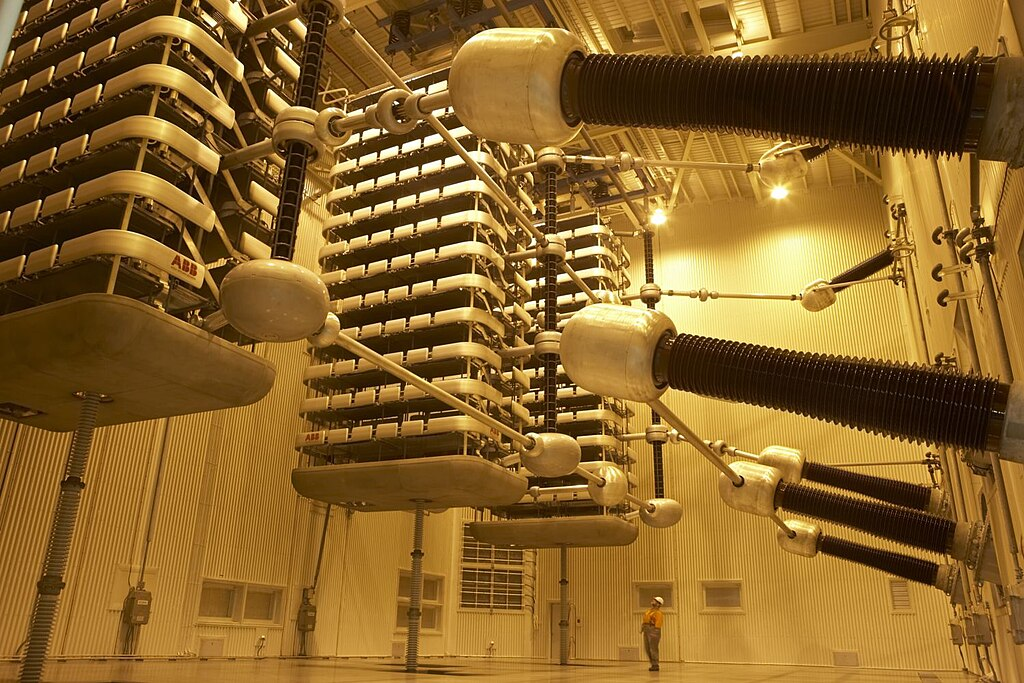
\includegraphics[width=0.5\textwidth]{fig/lec01/HVDC.jpg}
			\caption{High voltage DC transmission (source: \href{https://commons.wikimedia.org/wiki/File:Pole_2_Thyristor_Valve.jpg}{Wikimedia Commons},  	 	Marshelec, \href{https://creativecommons.org/licenses/by-sa/3.0/deed.en}{CC~BY-SA~3.0})}
		\end{subfigure}
	\end{figure}
\end{frame}

%%%%%%%%%%%%%%%%%%%%%%%%%%%%%%%%%%%%%%%%%%%%%%%%%%%%%%%%%%%%%
%% Power electronic application examples: transportation %%
%%%%%%%%%%%%%%%%%%%%%%%%%%%%%%%%%%%%%%%%%%%%%%%%%%%%%%%%%%%%%
\begin{frame}[c]
	\frametitle{Power electronic application examples: transportation}
	\begin{figure}
		\centering
		\begin{subfigure}[b]{0.49\textwidth}
			\centering
			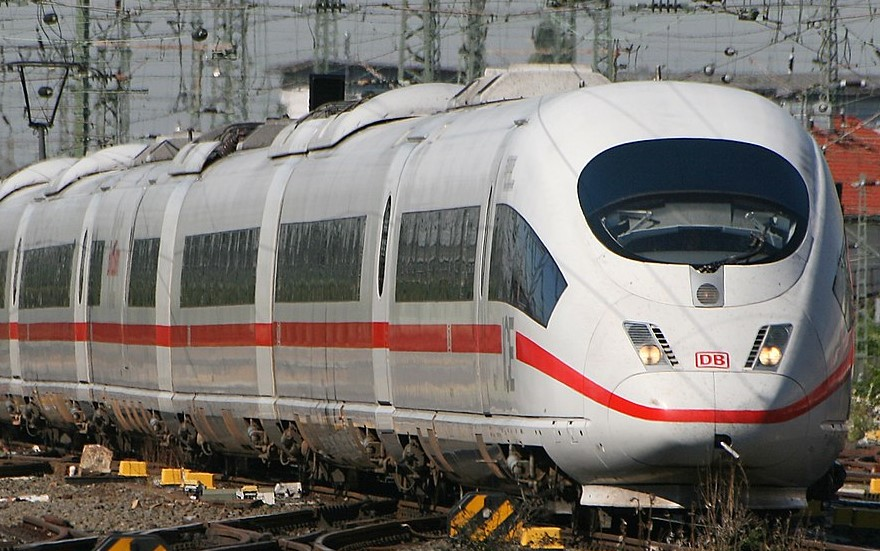
\includegraphics[width=0.5\textwidth]{fig/lec01/ICE.jpg}
			\caption{Train drive (source: \href{hhttps://commons.wikimedia.org/wiki/File:DB_AG_406_001-8.jpg}{Wikimedia Commons}, T.~Wolf, \href{https://creativecommons.org/publicdomain/zero/1.0/}{CC0~1.0})}
		\end{subfigure}
		\hfill
		\begin{subfigure}[b]{0.49\textwidth}
			\centering
			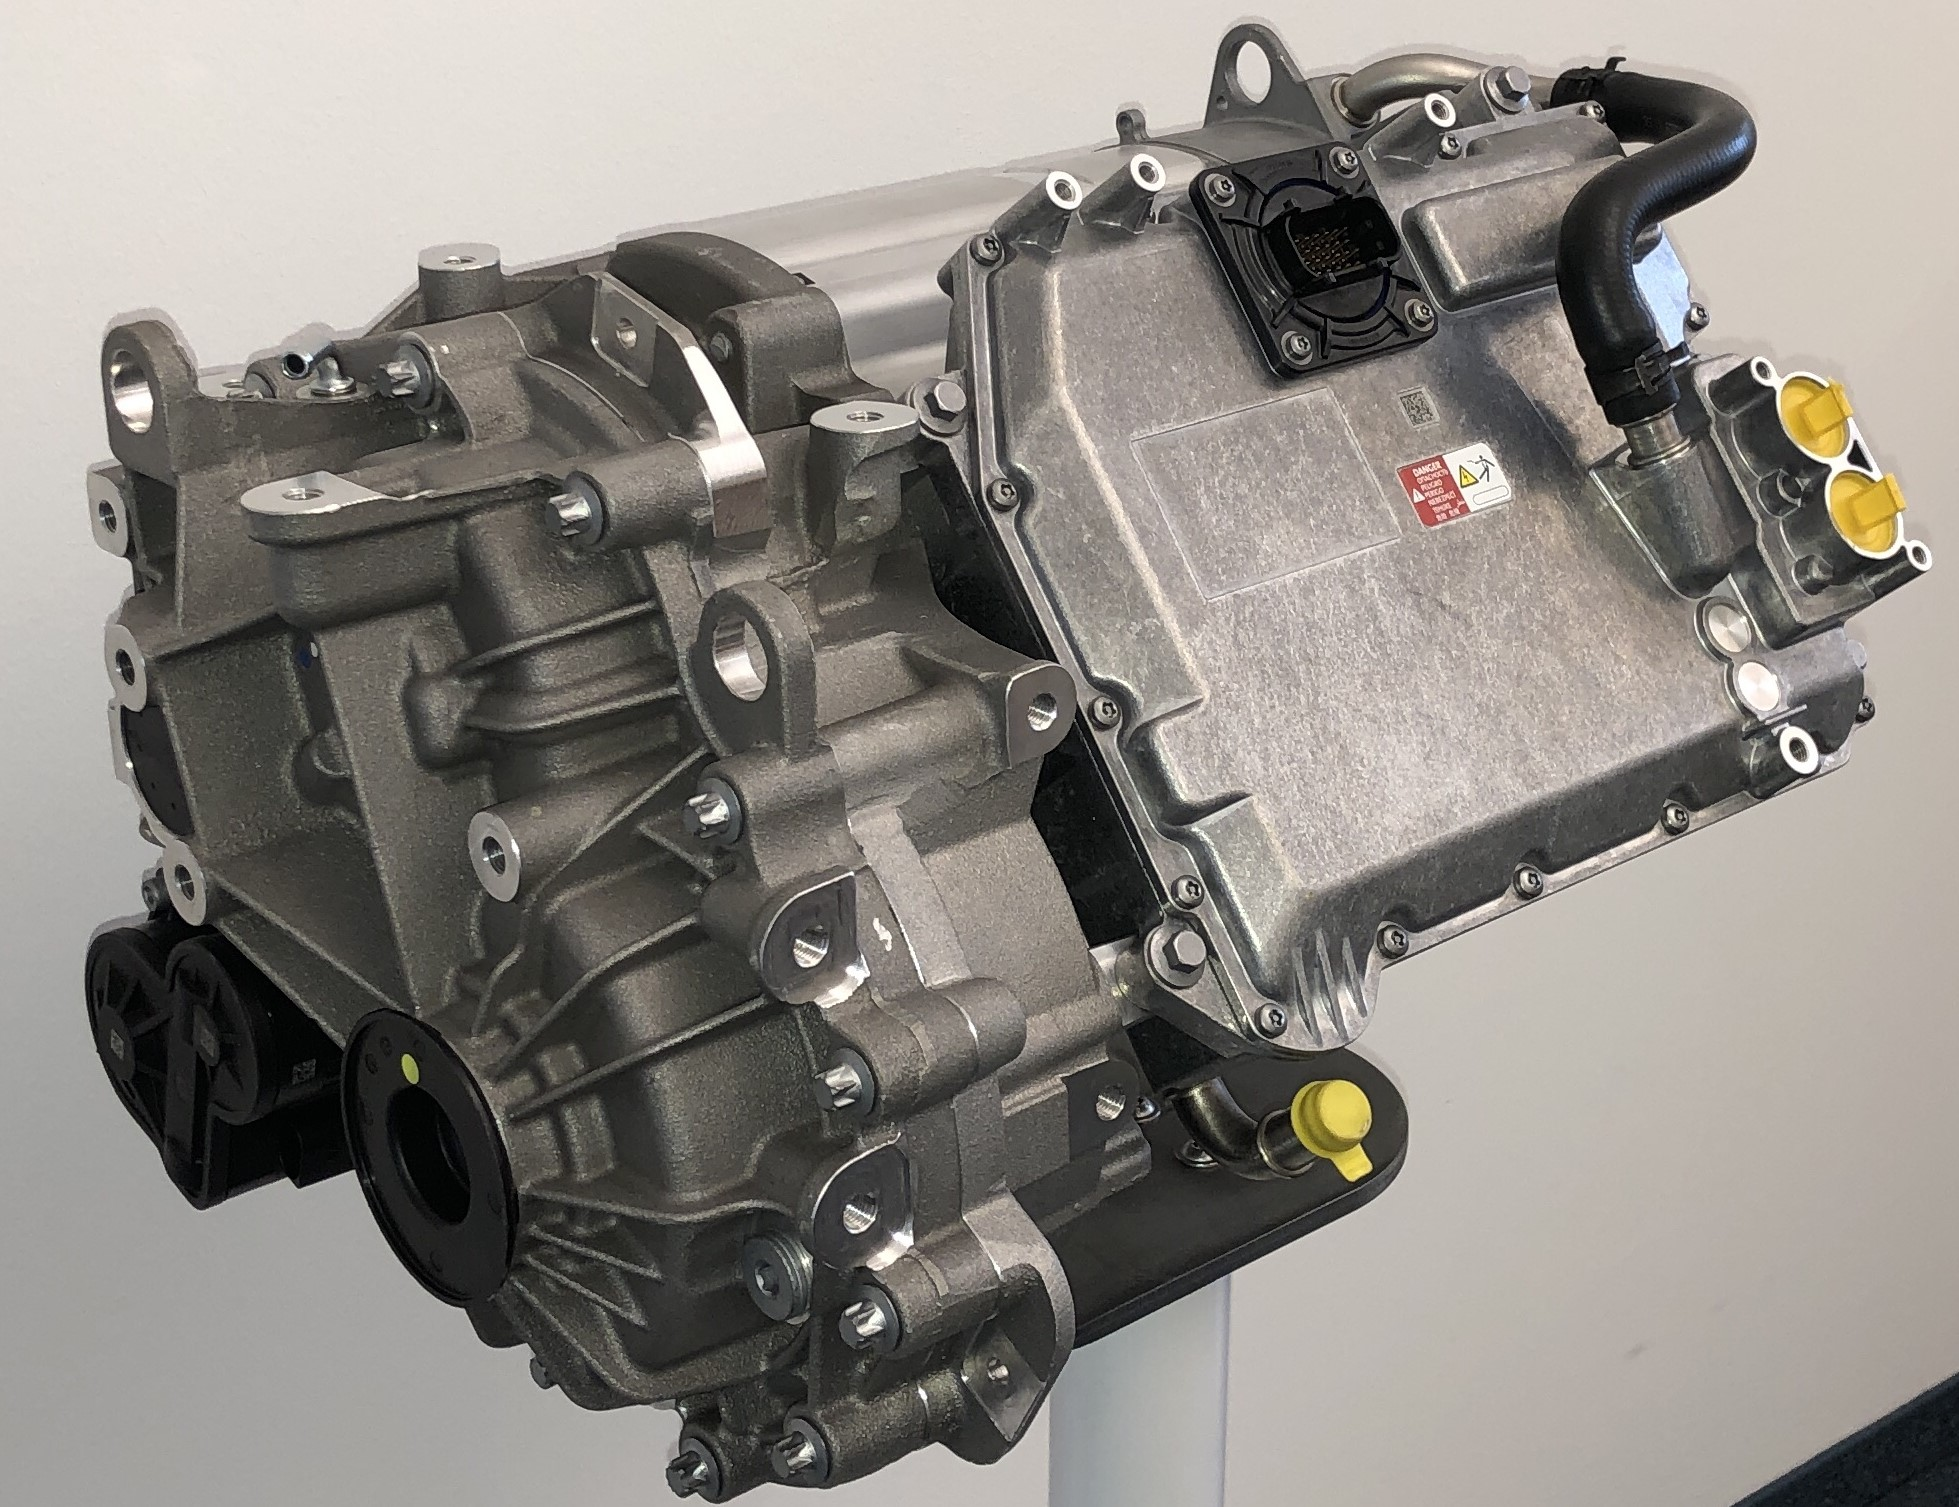
\includegraphics[width=0.5\textwidth]{fig/lec01/Drive.jpg}
			\caption{Electric vehicle drive (source: \href{https://commons.wikimedia.org/wiki/File:Vitesco_Technologies_EMR3.jpg}{Wikimedia Commons}, Caprolactam123, \href{https://creativecommons.org/licenses/by-sa/4.0/deed.en}{CC~BY-SA~4.0})}
		\end{subfigure}
		\\
		\begin{subfigure}[b]{0.49\textwidth}
			\centering
			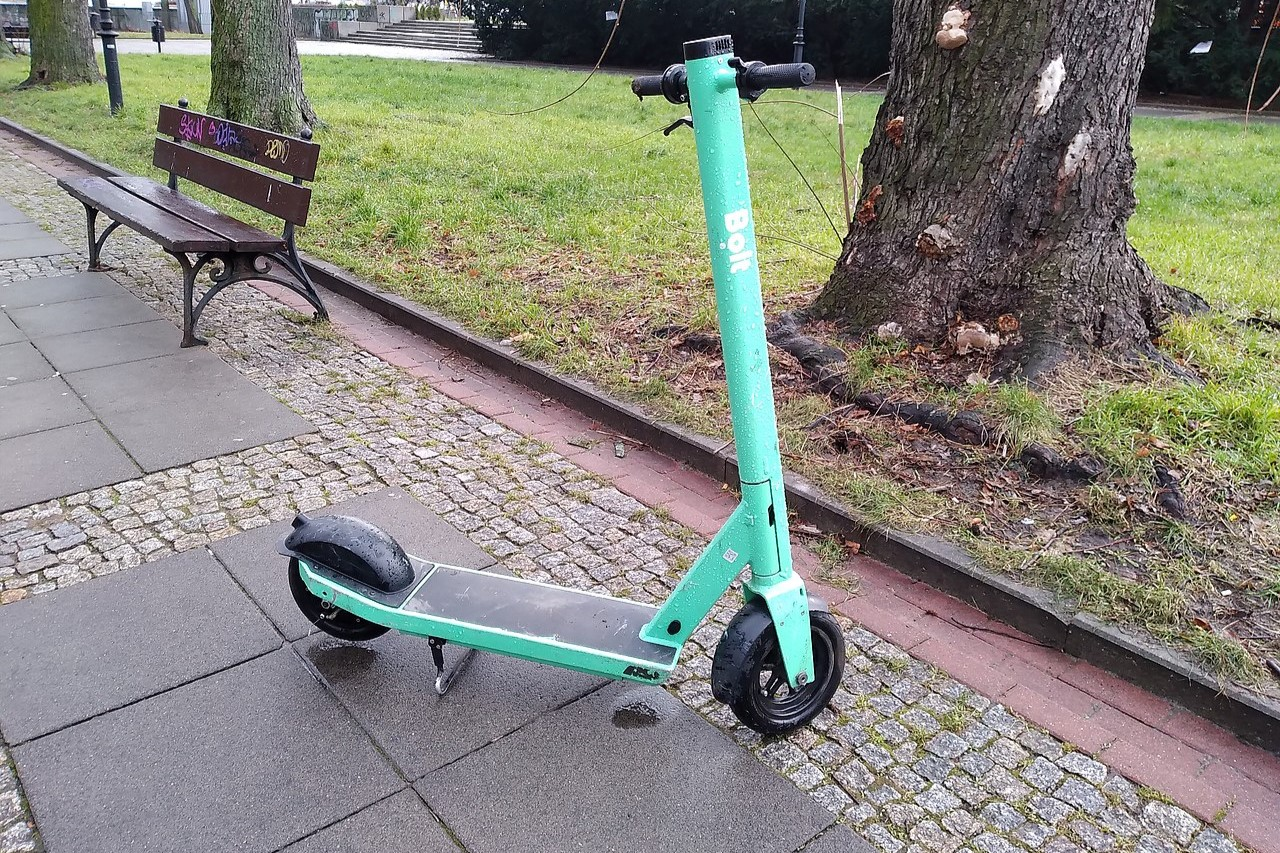
\includegraphics[width=0.5\textwidth]{fig/lec01/Scooter.jpg}
			\caption{Electric scooter (source: \href{https://commons.wikimedia.org/wiki/File:Bolt_Electric_Scooter_\%28Warsaw\%29_in_2020.03.jpg}{Wikimedia Commons}, Raju, \href{https://creativecommons.org/licenses/by-sa/4.0/deed.en}{CC~BY-SA~4.0})}
		\end{subfigure}
		\hfill
		\begin{subfigure}[b]{0.49\textwidth}
			\centering
			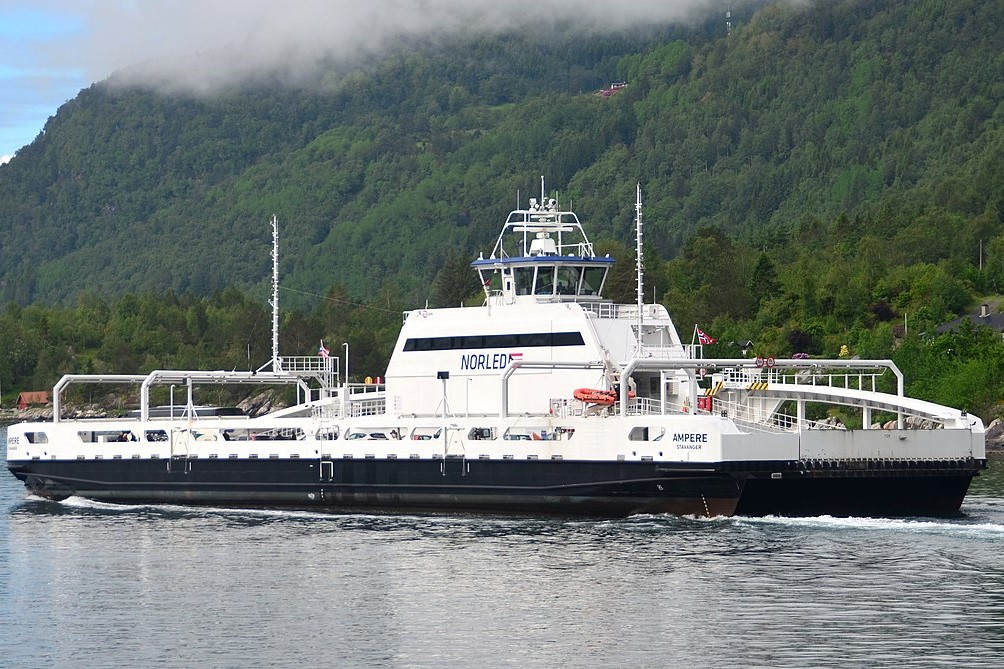
\includegraphics[width=0.5\textwidth]{fig/lec01/Electric_ship.jpg}
			\caption{Electic ship (source: \href{https://commons.wikimedia.org/wiki/File:Ferry_Ampere_Sognefjord.jpg}{Wikimedia Commons},  	 	Wikimalte, \href{https://creativecommons.org/licenses/by-sa/4.0/deed.en}{CC~BY-SA~4.0})}
		\end{subfigure}
	\end{figure}
\end{frame}

%%%%%%%%%%%%%%%%%%%%%%%%%%%%%%%%%%%%%%%%%%%%%%%%%%%%%%%%%%%%%
%% A broad range of nominal power ratings %%
%%%%%%%%%%%%%%%%%%%%%%%%%%%%%%%%%%%%%%%%%%%%%%%%%%%%%%%%%%%%%
\begin{frame}[c]
	\frametitle{A broad range of nominal power ratings}
	\vspace{0.3cm}
	\begin{figure}
		\centering
		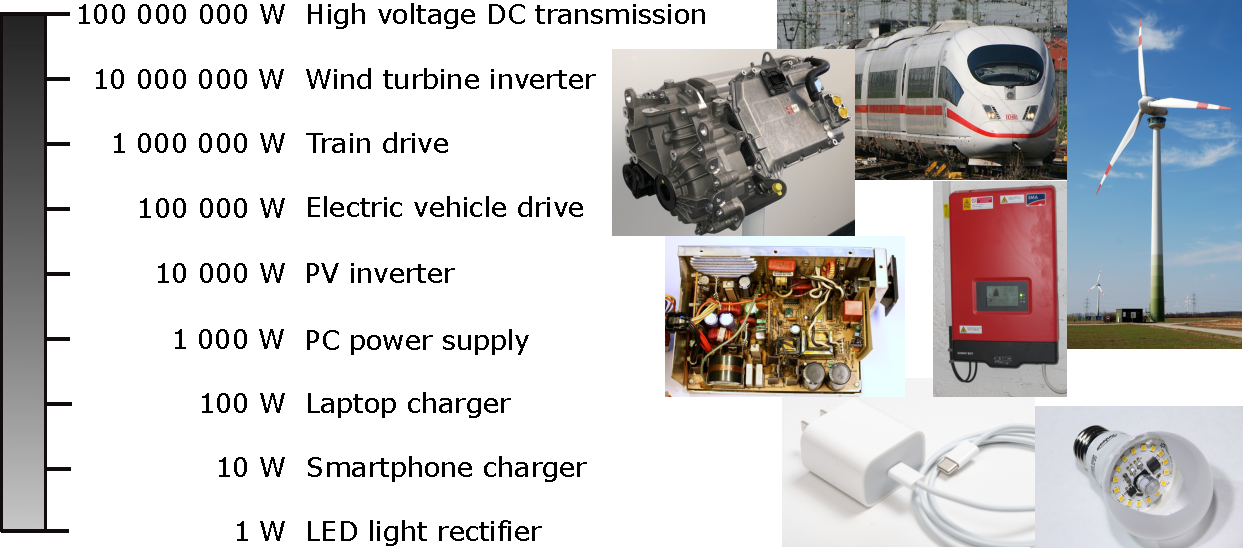
\includegraphics[height=0.7\textheight]{fig/lec01/Power_Classes_Examples.pdf}
		\caption{Power range overview (figure sources: \href{https://commons.wikimedia.org/wiki/File:DB_AG_406_001-8.jpg}{T. Wolf}, \href{https://commons.wikimedia.org/wiki/File:Wind_turbine_with_observation_deck_bruck_an_der_leitha.jpg}{KoeppiK}, \href{https://commons.wikimedia.org/wiki/File:Vitesco_Technologies_EMR3.jpg}{Caprolactam123}, \href{https://commons.wikimedia.org/wiki/File:Installation_of_solar_PV_panels_-_inverter_-_geograph.org.uk_-_2624304.jpg}{D. Hawgood}, \href{https://commons.wikimedia.org/wiki/File:IBM_PC_XT_5160_Power_Supply.jpg}{Mister rf}, \href{https://commons.wikimedia.org/wiki/File:LED-E27-Light-Bulb-1134.jpg}{D.~Tribble} and \href{https://www.rawpixel.com/image/5923136/photo-image-phone-public-domain-white}{rawpixel} under varying CC licenses) }
		\label{Power_Classes_Examples}
	\end{figure}
\end{frame}

%%%%%%%%%%%%%%%%%%%%%%%%%%%%%%%%%%%%%%%%%%%%%%%%%%%%%%%%%%%%%
%% Typical power electronic objectives %%
%%%%%%%%%%%%%%%%%%%%%%%%%%%%%%%%%%%%%%%%%%%%%%%%%%%%%%%%%%%%%
\begin{frame}[c]
	\frametitle{Typical power electronic objectives}
	\begin{figure}
		\begin{tikzpicture}
			\begin{axis}[
				height=.70\textheight,
				ylabel={Efficiency},
				xlabel={Power density},
				zlabel={Costs / ressources},
				xlabel style={sloped},
				ylabel style={sloped}, 
				xticklabel style = {yshift=0.2cm, rotate=25},
				view={70}{25},
				grid,
				ymax = 1,
				xmax = 1,
				zmax = 1,
				xtick distance = 0.25,
				ytick distance = 0.25,
				ztick distance = 0.25
			]
			\addplot3[
				mesh,
				samples=20,
				domain=0:1,
				draw = signalblue
			](
				{sqrt(1-x^2) * cos(deg(y))},
				{sqrt( 1-x^2 ) * sin(deg(y))},
				{x}
			);
			\end{axis}
		\end{tikzpicture}
		\caption{Illustration of typical, conflicting power electronic (normalized) objectives via a Pareto front}
		\label{fig:power_electronic_objectives}
	\end{figure}
\end{frame}

%%%%%%%%%%%%%%%%%%%%%%%%%%%%%%%%%%%%%%%%%%%%%%%%%%%%%%%%%%%%%
%% Terminology: work vs. energy%%
%%%%%%%%%%%%%%%%%%%%%%%%%%%%%%%%%%%%%%%%%%%%%%%%%%%%%%%%%%%%%
\begin{frame}[c]
	\frametitle{Terminology: work vs. energy}
	\begin{columns}
		\begin{column}{0.5\textwidth}
			\begin{varblock}{Work}
				Work is the integral of the power over a time integral (or force over distance) and is a measure of the energy transfer.
			\end{varblock}
		\end{column}
		\begin{column}{0.5\textwidth}
			\begin{varblock}{Energy}
				Energy is the capacity to do work, that is, a quantity depending on the state of a system at a given point of time.				
			\end{varblock}
		\end{column}
	\end{columns}
	\vspace{0.5cm}
	\begin{figure}
		\begin{tikzpicture}
			\node[draw, bubble, minimum width = 8em, minimum height = 5em] (energy) at (0,0) {\large Energy};
			\coordinate (loss) at (4.5,-1.25);
			\node[draw, bubble] (energy2) at (6,0) {\large Energy};
			\begin{scope}[on background layer]
				\draw[-{Latex[length=4mm, width=8mm]}, line width=4mm] (energy.mid) -- node[above, midway, name = work] {Work} (energy2);
				\draw[-{Latex[length=4mm, width=8mm]}, line width=2mm, color=signalred, transform canvas={yshift=-3mm}] (energy.mid) --  (3,0) to [out=0,in=120] (loss.south) ;
				\node[below, transform canvas={yshift=-3mm}] at (loss) {\color{signalred} \large Heat};
				\node[below=of work, yshift = 6mm, color=signalred] {Losses};
			\end{scope}
		\end{tikzpicture}
		\vspace{0.75cm}
		\caption{Illustration addressing the work vs. energy terminology (simplified Sankey diagram)}
		\label{fig:work_vs_energy}
	\end{figure}
\end{frame}

%%%%%%%%%%%%%%%%%%%%%%%%%%%%%%%%%%%%%%%%%%%%%%%%%%%%%%%%%%%%%
%% Power Power balance of an electrical energy conversion system %%
%%%%%%%%%%%%%%%%%%%%%%%%%%%%%%%%%%%%%%%%%%%%%%%%%%%%%%%%%%%%%
\begin{frame}
	\frametitle{Power balance of an electrical energy conversion system}
	\begin{figure}
		\begin{tikzpicture}[auto, node distance = 1.5cm and 2cm]
			\draw
				node [input, name = input] {}
				node [bubble, right = of input, minimum height = 4em, pin=80:Change of stored energy $ \frac{\mathrm{d}}{\mathrm{d}t}E_\mathrm{i}(t)$] (pc) {\large Power converter}
				node [output, name = output, right = of pc] {}
				node [output, name = losses, below = of pc] {};
			\draw[-{Latex[length=4mm, width=8mm]}, line width=3mm] (input) -- node[below, midway, align=left, name = input2] {Electrical\\input power} (pc);
			\begin{scope}[on background layer]
				\draw[-{Latex[length=4mm, width=8mm]}, line width=3mm] (pc.mid) -- node[below, near end, align=left, name=output2] {Electrical\\output power} (output);
				\draw[-{Latex[length=4mm, width=8mm]}, line width=3mm, color=signalred] (pc.mid) -- node[right, yshift=-2.5mm, name = losses2] {Losses} (losses);
			\end{scope}
			\node[left=of losses2, color=signalred, xshift = 1.8cm] {$P_\mathrm{l}(t)$};
			\node[above=of output2.mid,, align=center, xshift = -0.3cm, yshift = -5mm] {$P_\mathrm{out}(t)$};
			\node[above=of input2.mid,, align=center, xshift = -0.3cm, yshift = -5mm] {$P_\mathrm{in}(t)$};
		\end{tikzpicture}
		\caption{Power balance of an energy conversion system}
		\label{fig:power_balance_energy_conversion}
	\end{figure}
	\vspace{-0.5cm}
	The \hl{power balance}
	\begin{equation}
		P_\mathrm{in}(t) = P_\mathrm{out}(t) + P_\mathrm{l}(t) + \frac{\mathrm{d}}{\mathrm{d}t}E_\mathrm{i}(t)
	\end{equation}
	must hold for any point in time as energy is conserved, that is, not created or destroyed.
\end{frame}

%%%%%%%%%%%%%%%%%%%%%%%%%%%%%%%%%%%%%%%%%%%%%%%%%%%%%%%%%%%%%
%% Efficiency %%
%%%%%%%%%%%%%%%%%%%%%%%%%%%%%%%%%%%%%%%%%%%%%%%%%%%%%%%%%%%%%
\begin{frame}
	\frametitle{Efficiency}
	\begin{figure}
		\begin{tikzpicture}[auto, node distance = 1.5cm and 2cm]
			\draw
				node [input, name = input] {}
				node [bubble, right = of input, minimum height = 4em] (pc) {\large Power converter}
				node [output, name = output, right = of pc] {}
				node [output, name = losses, below = of pc] {};
			\draw[-{Latex[length=4mm, width=8mm]}, line width=3mm] (input) -- node[below, midway, align=left, name = input2] {Electrical\\input power} (pc);
			\begin{scope}[on background layer]
				\draw[-{Latex[length=4mm, width=8mm]}, line width=3mm] (pc.mid) -- node[below, near end, align=left, name=output2] {Electrical\\output power} (output);
				\draw[-{Latex[length=4mm, width=8mm]}, line width=3mm, color=signalred] (pc.mid) -- node[right, yshift=-2.5mm, name = losses2] {Losses} (losses);
			\end{scope}
			\node[left=of losses2, color=signalred, xshift = 1.8cm] {$P_\mathrm{l}$};
			\node[above=of output2.mid,, align=center, xshift = -0.3cm, yshift = -5mm] {$P_\mathrm{out}$};
			\node[above=of input2.mid,, align=center, xshift = -0.3cm, yshift = -5mm] {$P_\mathrm{in}$};
		\end{tikzpicture}
		\caption{Power balance of an energy conversion system in steady state}
		\label{fig:power_balance_energy_conversion_steady_state}
	\end{figure}
	\vspace{-0.5cm}
	The power balance in steady state ($\nicefrac{\mathrm{d}x(t)}{\mathrm{d} t}=0$) is
	\begin{equation}
		P_\mathrm{in} = P_\mathrm{out} + P_\mathrm{l}
	\end{equation}
	and leads to the definition of the \hl{efficiency}
	\begin{equation}
		\eta = \frac{P_\mathrm{out}}{P_\mathrm{in}} = \frac{P_\mathrm{out}}{P_\mathrm{out} + P_\mathrm{l}}.
	\end{equation}
\end{frame}

%%%%%%%%%%%%%%%%%%%%%%%%%%%%%%%%%%%%%%%%%%%%%%%%%%%%%%%%%%%%%
%% Why efficiency matters: a computer supply example %%
%%%%%%%%%%%%%%%%%%%%%%%%%%%%%%%%%%%%%%%%%%%%%%%%%%%%%%%%%%%%%
\begin{frame}[c]
	\frametitle{Why efficiency matters: a computer supply example}
	\begin{table}
		\centering
		\begin{tabular}{lcc}
			\toprule
			& Power supply A & Power supply B \\
			& 80 PLUS Gold & 80 PLUS Titanium \\
			\midrule
			Input power & \multicolumn{2}{c}{\SI{250}{\watt}} \\
			Efficiency & \SI{89}{\percent} & \SI{94}{\percent}  \\
			Power loss & \SI{27.5}{\watt} & \SI{15}{\watt}\\
			\midrule
			Operating hours per year & \multicolumn{2}{c}{$\SI{8}{\hour} \times 220 = \SI{1760}{\hour}$} \\
			Cumulated power loss per year & \SI{48.4}{\kilo\watt\hour} & \SI{26.4}{\kilo\watt\hour} \\
			Electricity cost for yearly power losses & \SI{14.52}{\EUR} & \SI{7.92}{\EUR} \\
			\midrule
			Cumulated power loss in Germany & \SI{1.936}{\tera\watt\hour} & \SI{1.056}{\tera\watt\hour} \\
			Electricity cost for power loss in Germany & \SI{580.8}{\mega\EUR} & \SI{316.8}{\mega\EUR} \\
			\bottomrule
		\end{tabular}
		\label{tab:efficiency_computer_supply_example}
		\caption{Comparison of two computer power supplies (further assumptions: effective nominal power calculation, electricity price \SI[fraction-function=\nicefrac]{0.3}{\EUR\per\kilo\watt\per\hour}, $40\cdot 10^6$ computers in Germany)}
	\end{table}
\end{frame}

%%%%%%%%%%%%%%%%%%%%%%%%%%%%%%%%%%%%%%%%%%%%%%%%%%%%%%%%%%%%%
%% Why efficiency matters: a wind power plant example %%
%%%%%%%%%%%%%%%%%%%%%%%%%%%%%%%%%%%%%%%%%%%%%%%%%%%%%%%%%%%%%
\begin{frame}[c]
	\frametitle{Why efficiency matters: a wind power plant example}
	\begin{table}
		\centering
		\begin{tabular}{lcc}
			\toprule
			& Wind power plant A & Wind power plant B \\
			\midrule
			Input power & \multicolumn{2}{c}{\SI{5}{\mega\watt}} \\
			Efficiency & \SI{97}{\percent} & \SI{97.1}{\percent}  \\
			Power loss & \SI{150}{\kilo\watt} & \SI{145}{\kilo\watt}\\
			\midrule
			Nominal power operating hours per year & \multicolumn{2}{c}{$\SI{3000}{\hour}$} \\
			Cumulated power loss per year & \SI{450}{\mega\watt\hour} & \SI{435}{\mega\watt\hour} \\
			Cumulated power loss (lifetime) & \SI{9.0}{\giga\watt\hour} & \SI{8.7}{\giga\watt\hour} \\
			\midrule
			Lost sales proceeds due to losses per year  & \SI{22.5}{\kilo\EUR} & \SI{21.75}{\kilo\EUR} \\
			Lost sales proceeds due to losses (lifetime)  & \SI{450}{\kilo\EUR} & \SI{435}{\kilo\EUR} \\
			\midrule
			Cumulated power loss (lifetime, Germany)  & \SI{9.0}{\tera\watt\hour} & \SI{8.7}{\tera\watt\hour} \\
			Lost sales proceeds (lifetime, Germany)  & \SI{450}{\mega\EUR} & \SI{435}{\mega\EUR} \\
			\bottomrule
		\end{tabular}
		\label{tab:efficiency_wind_power_example}
		\caption{Comparison of two wind power plants (further assumptions:  electricity sales price \SI[fraction-function=\nicefrac]{0.05}{\EUR\per\kilo\watt\per\hour}, $20$ years of life time, $\num{1000}$ newly constructed wind power plants per year in Germany)}
	\end{table}
\end{frame}


%%%%%%%%%%%%%%%%%%%%%%%%%%%%%%%%%%%%%%%%%%%%%%%%%%%%%%%%%%%%%
%% Linear power conversion %%
%%%%%%%%%%%%%%%%%%%%%%%%%%%%%%%%%%%%%%%%%%%%%%%%%%%%%%%%%%%%%
\begin{frame}[c]
	\frametitle{Linear power conversion}
	\begin{figure}
		\begin{circuitikz}[]
			\draw (0,2) to [open, o-o, v = $\hspace{2cm}u_\mathrm{out}(t)$, voltage = straight] ++(0,-2)
			to ++(-6,0)
			to [open, o-o, v<= $u_\mathrm{in}(t) \hspace{2cm}$, voltage = straight] ++(0,2)
			to [european resistor, R=$R_1$] ++(4,0) 
			to ++(2,0)
			(-2,0) to [variable european resistor, *-*, l=$R_2$] (-2,2);
		\end{circuitikz}
		\caption{Adjustable resistive voltage divider as step-down converter}
		\label{fig:linear_power_conversion}
	\end{figure}
	With Kirchhoff's voltage law, the output voltage $u_\mathrm{out}(t)$ is
	\begin{equation}
		u_\mathrm{out}(t) = u_\mathrm{in}(t) \frac{R_2}{R_1 + R_2}.
	\end{equation}
	By adjusting the resistance $R_2$, the output voltage can be controlled. However, this method is \hl{inefficient} as the power loss is independent of the output power and given by
	\begin{equation}
		P_\mathrm{l}(t) = \frac{u_\mathrm{in}^2(t)}{R_1 + R_2}.
	\end{equation}
\end{frame}

%%%%%%%%%%%%%%%%%%%%%%%%%%%%%%%%%%%%%%%%%%%%%%%%%%%%%%%%%%%%%
%% Linear power conversion (cont.) %%
%%%%%%%%%%%%%%%%%%%%%%%%%%%%%%%%%%%%%%%%%%%%%%%%%%%%%%%%%%%%%
\begin{frame}[c]
	\frametitle{Linear power conversion (cont.)}
	\begin{columns}
		\begin{column}{0.55\textwidth}
			\begin{figure}
				\begin{circuitikz}[]
					\draw (0,2) to [open, o-o, v = $\hspace{2cm}u_\mathrm{out}(t)$, voltage = straight] ++(0,-2)
					to ++(-5.5,0)
					to [open, o-o, v<= $u_\mathrm{in}(t) \hspace{2cm}$, voltage = straight] ++(0,2)
					(-5.5,2) to ++(1.25,0) node [nigbt, anchor=C, rotate=90](nigbt1){}
					(nigbt1.E) to [short, i=$i_\mathrm{out}(t)$] (0,2);
					\draw node[rectangle, draw, anchor = north] (r) at (nigbt1.B) {Linear amplifier}
						(r.east)[<-] to ++(0.5,0) node [anchor = west](a){$u^*_\mathrm{out}(t)$};
					\draw [->] ([yshift = 0.2cm, xshift = 0.1cm]nigbt1.C) -- node [yshift = 0.3cm] {$u_\mathrm{CE}(t)$} ([yshift = 0.2cm, xshift = -0.1cm]nigbt1.E) ;  
				\end{circuitikz}
				\caption{Transistor-based step-down converter}
				\label{fig:linear_power_conversion_transistor}
			\end{figure}
			For a transistor-based step-down converter, the output voltage  is $u_\mathrm{out}(t)= u_\mathrm{in}(t) - u_\mathrm{CE}(t)$	leading to the power losses
			\begin{equation}
				P_\mathrm{l}(t) = u_\mathrm{CE}(t)  i_\mathrm{out}(t) .
			\end{equation}
		\end{column}
		\begin{column}{0.45\textwidth}
			\centering
			\begin{figure}
				\begin{tikzpicture}
					% plot IGBT output characteristics V_CE = f(I_C)
					\begin{axis}[
						xlabel={$U_{\mathrm{CE}}$},
						ylabel={$I_\mathrm{C}$},
						axis lines=left,
						ymin=0, ymax=6,
						xmin=0, xmax=5,
						xtick={0,1,2,3,4},
						ytick={0,1,2,3,4,5},
						%no x/y ticks displayed
						xticklabels={},
						yticklabels={},
						domain=0:5,
						samples=50,
						thick,
						smooth,
						no markers,
						width = 0.95\textwidth,
						grid
						]
						% plt IGBT output characteristics consider the linear, saturation and cut-off region
						\addplot[signalblue, domain=0:0.3]{0.01};
						\addplot[signalblue, domain=0.3:5]{11.5 / (1+exp(-2*(x-0.3)))-6};
						\addplot[signalblue, domain=0.3:5]{7.7 / (1+exp(-2.5*(x-0.3)))-4};
						\addplot[signalblue, domain=0.3:5]{4 / (1+exp(-3*(x-0.3)))-2};
						\addplot[signalblue, domain=0.3:5]{2 / (1+exp(-3.25*(x-0.3)))-1};
						\addplot[signalblue, domain=0.3:5]{1 / (1+exp(-3.5*(x-0.325)))-0.5};
						\addplot[signalblue, domain=0.3:5]{0.25 / (1+exp(-3.5*(x-0.325)))-0.125};

						% arrow pointing upwards at x = 4 to indicate the dependance on U_GE
						\draw[->, signalbrown, thick, dashed] (axis cs:1.5,0.25) -- (axis cs:1.5,5.2);
						\node[signalbrown, anchor = west] at (axis cs:1.5,2.75) {$U_\mathrm{GE}$};
						% plot a ellipse shape in the background of the linear region
						\draw[signalgreen, thick, dashed, rotate=-10] (axis cs:0.5,1) ellipse (0.35cm and 3.0cm);
						\node[signalgreen, anchor = south] at (axis cs:1.1,5.1) {\small Linear region};

						%add a rectangle with rounded corners around the saturation area
						\draw[signalred, thick, dashed, rounded corners] (axis cs:2.5,0.2) rectangle (axis cs:4.75,5.9);
						\node[signalred, anchor = south, ,  align=center] at (axis cs:3.6,3.7) {\small Saturation\\region};
					\end{axis}
				\end{tikzpicture}
				\caption{Output characteristics of an insulated-gate bipolar transistor}
				\label{fig:output_characteristics_IGBT}
			\end{figure}
			\end{column}
	\end{columns}
\end{frame}

%%%%%%%%%%%%%%%%%%%%%%%%%%%%%%%%%%%%%%%%%%%%%%%%%%%%%%%%%%%%%
%% Switching power conversion %%
%%%%%%%%%%%%%%%%%%%%%%%%%%%%%%%%%%%%%%%%%%%%%%%%%%%%%%%%%%%%%
\begin{frame}[b]
	\frametitle{Switching power conversion}
	Alternative idea: \hl{switch either fully on or off}. The average output voltage $\overline{u}_\mathrm{out}$ is controlled by the duty cycle (assuming that $u_\mathrm{in}(t)=\overline{u}_\mathrm{in}$ is constant)
	\begin{equation}
		D = \frac{T_\mathrm{on}}{T_\mathrm{s}}, \qquad \overline{u}_\mathrm{out} = \frac{1}{T_\mathrm{s}} \int_0^{T_\mathrm{s}} u_\mathrm{out}(t) \mathrm{d}t = D \overline{u}_\mathrm{in}.
	\end{equation}
	As the switching losses are typically small, the overall efficiency is (much) higher compared to linear power conversion. 
	\vspace{-0.5cm}  
	\begin{columns}[b]
		\begin{column}{0.5\textwidth}
			\begin{figure}
				\begin{circuitikz}[]
					\draw (0,2) to [open, o-o, v = $\hspace{2cm}u_\mathrm{out}(t)$, voltage = straight] ++(0,-2)
					to ++(-5,0)
					to [open, o-o, v<= $u_\mathrm{in}(t) \hspace{2cm}$, voltage = straight] ++(0,2)
					(-5,2) to ++(1.25,0) node [cuteopenswitchshape, anchor = out, rotate=180] (S) {}
					let \p1 = (S.mid) in (S.in) to (0,2)
					([yshift = -0.3cm]S.mid) to [short, o-*](\x1,0);
				\end{circuitikz}
				\vspace{0.6cm}
				\caption{Ideal switch-based step-down converter}
				\label{fig:Switched_power_conversion}
			\end{figure}
			\vspace{0pt}
		\end{column}
		\begin{column}{0.5\textwidth}
			\centering
			\begin{figure}
				\begin{tikzpicture}
					% plot switching output voltage with an ideal switch between u_out = u_int for t = 0 D*Ts and u_out = 0 for t = D*Ts to Ts
					\begin{axis}[
						xlabel={$t/T_\mathrm{s}$},
						ylabel={$u_\mathrm{out}(t)/u_\mathrm{in}(t)$},
						ymin=-0.05, ymax=1.05,
						xmin=-0.1, xmax=1.1,
						width = 0.95\textwidth,
						height = 0.4\textheight,
						grid,
						thick,
						clip = false,
						]
						% plt u_out = 1 for t = 0 to D*Ts and u_out = 0 for t = D*Ts to Ts in a single plot
						\addplot[signalblue] coordinates {(-0.1,0) (0,0) (0,1) (0.4,1) (0.4,0) (1,0) (1,1) (1.1,1)};
						\draw [thick,<->]  (0,0.5) -- node[above,fill=white]{$T_\mathrm{on}$}(0.4, 0.5); 
						\draw [thick,<->]  (0.4,0.5) -- node[above]{$T_\mathrm{off}$}(1.0, 0.5);
						\draw [thick,<->]  (0.0,1.2) -- node[above]{$T_\mathrm{s}$}(1.0, 1.2); 
					\end{axis}
				\end{tikzpicture}
				\caption{Switching output voltage from \figref{fig:Switched_power_conversion}}
				\label{fig:Switched_power_conversion_output}
			\end{figure}
			\vspace{0pt}
			\end{column}
	\end{columns}
\end{frame}

%%%%%%%%%%%%%%%%%%%%%%%%%%%%%%%%%%%%%%%%%%%%%%%%%%%%%%%%%%%%%
%% Important power electronic devices %%
%%%%%%%%%%%%%%%%%%%%%%%%%%%%%%%%%%%%%%%%%%%%%%%%%%%%%%%%%%%%%
\begin{frame}[c]
	\frametitle{Important power electronic devices}
\begin{table}
	\begin{tabular}{M{0.22\textwidth} M{0.22\textwidth} M{0.22\textwidth} M{0.22\textwidth}}
		Diode & Bipolar junction transistor & MOSFET\footnote{metal-oxide-semiconductor field-effect transistor} (with body diode) & Thyristor \\
		\begin{circuitikz}
			\draw (0,0) to [diode, v=$u$, i=$i$, , voltage = straight] (2,0);
		\end{circuitikz}
		&
		\begin{circuitikz}
			\draw (0,0) to [short, i=$i$, xshift = 0.1cm] ++(0.25,0) 
			to ++(0.01,0)  node [npn, anchor=C, rotate=90](npn1){}
			(npn1.E) to [short] (2,0);
			\draw [->] ([yshift = 0.2cm, xshift = 0.1cm]npn1.C) -- node [yshift = 0.25cm] {$u$} ([yshift = 0.2cm, xshift = -0.1cm]npn1.E) ;
		\end{circuitikz}
		&
		\begin{circuitikz}
			\draw (0,0) to [short, i=$i$, xshift = 0.1cm] ++(0.25,0) 
			to ++(0.01,0)  node [nigfete, anchor=D, rotate=90, bodydiode](fet1){}
			(fet1.S) to [short] (2,0);
			\draw [->] ([yshift = 0.5cm, xshift = 0.1cm]fet1.D) -- node [yshift = 0.3cm] {$u$} ([yshift = 0.5cm, xshift = -0.1cm]fet1.S) ;
		\end{circuitikz}
		&
		\begin{circuitikz}
			\draw (0,0) to node[emptythyristorshape](ty1){} (2,0);
			\draw (ty1.cathode) to [short, i_=$i$, , xshift = -0.2cm] (2,0);
			\draw [->] ([yshift = -0.5cm, xshift = 0.1cm]ty1.anode) -- node [yshift = -0.3cm] {$u$} ([yshift = -0.5cm, xshift = -0.1cm]ty1.cathode) ;
		\end{circuitikz}		
		\\

		\begin{tikzpicture}
			\begin{axis}[
				xmin=-1, xmax=1,
				ymin=-1, ymax=1,
				width=0.25\textwidth,
				height=0.5\textheight,
				axis lines=middle,
				clip = false,
				thick,
				xlabel = {$u$},
				ylabel = {$i$},
				xticklabels=\empty,
				xlabel style={anchor = west},
				ylabel style={anchor = north east},
				yticklabels=\empty,
				anchor = center
				]
				\addplot[signalred, very thick] coordinates {(-1,0) (0,0) (0,1)};
			\end{axis}
		\end{tikzpicture}

		&

		\begin{tikzpicture}
			\begin{axis}[
				xmin=-1, xmax=1,
				ymin=-1, ymax=1,
				width=0.25\textwidth,
				height=0.5\textheight,
				axis lines=middle,
				clip = false,
				thick,
				xlabel = {$u$},
				ylabel = {$i$},
				xticklabels=\empty,
				xlabel style={anchor = west},
				ylabel style={anchor = north east},
				yticklabels=\empty,
				anchor = center
				]
				\addplot[signalred, very thick] coordinates {(0,0) (1,0)};
				\addplot[signalgreen, very thick] coordinates {(0,0) (0,1)};
				%\node[pin= left:{\footnotesize\color{signalgreen}active\\gate}, align=right] at (axis cs:0,0.5) {};
				\draw [pin] (axis cs:-0.05,0.5) -- +(-10pt,-5pt) node[left, align=center, font=\footnotesize ] {active\\ gate};
				\draw [pin] (axis cs:0.25,-0.05) -- +(12pt,-10pt) node[below, align=center, font=\footnotesize ] {disabled\\ gate};
			\end{axis}
		\end{tikzpicture}

		&

		\begin{tikzpicture}
			\begin{axis}[
				xmin=-1, xmax=1,
				ymin=-1, ymax=1,
				width=0.25\textwidth,
				height=0.5\textheight,
				axis lines=middle,
				clip = false,
				thick,
				xlabel = {$u$},
				ylabel = {$i$},
				xticklabels=\empty,
				xlabel style={anchor = west},
				ylabel style={anchor = north east},
				yticklabels=\empty,
				anchor = center
				]
				\addplot[signalred, very thick] coordinates {(0,0) (1,0)};
				\addplot[signalgreen, very thick] coordinates {(0,-1) (0,1)};
				%\node[pin= left:{\footnotesize\color{signalgreen}active\\gate}, align=right] at (axis cs:0,0.5) {};
				\draw [pin] (axis cs:-0.05,0.5) -- +(-10pt,-5pt) node[left, align=center, font=\footnotesize ] {active\\ gate};
				\draw [pin] (axis cs:0.25,-0.05) -- +(10pt,-10pt) node[below, align=center, font=\footnotesize ] {disabled\\ gate};
				\draw [pin] (axis cs:-0.05,-0.5) -- +(-12pt,5pt) node[left, align=center, font=\footnotesize ] {body\\ diode};
			\end{axis}
		\end{tikzpicture}

		&

		\begin{tikzpicture}
			\begin{axis}[
				xmin=-1, xmax=1,
				ymin=-1, ymax=1,
				width=0.25\textwidth,
				height=0.5\textheight,
				axis lines=middle,
				clip = false,
				thick,
				xlabel = {$u$},
				ylabel = {$i$},
				xticklabels=\empty,
				xlabel style={anchor = west},
				ylabel style={anchor = north east},
				yticklabels=\empty,
				anchor = center
				]
				\addplot[signalred, very thick] coordinates {(0,0) (1,0)};
				\addplot[signalgreen, very thick] coordinates {(0,0) (0,1)};
				%\node[pin= left:{\footnotesize\color{signalgreen}active\\gate}, align=right] at (axis cs:0,0.5) {};
				\draw [pin] (axis cs:-0.05,0.5) -- +(-10pt,-5pt) node[left, align=center, font=\footnotesize ] {active\\ gate};
				\draw [pin] (axis cs:0.05,0.5) -- +(10pt,-5pt) node[right, align=center, font=\footnotesize ] {no turn\\off};
				\draw [pin] (axis cs:0.25,-0.05) -- +(12pt,-10pt) node[below, align=center, font=\footnotesize ] {disabled\\ gate};
			\end{axis}
		\end{tikzpicture}

	\end{tabular}
\end{table}
\end{frame}
